%% LLT: Turn off some annoying warnings...
\RequirePackage{silence}
\WarningFilter{titlesec}{Non standard sectioning command}
\WarningFilter{scrreprt}{Usage of package}
\WarningFilter{scrreprt}{Activating an ugly workaround}

% **************************************************
% Document Class Definition
% **************************************************
\documentclass[%
	paper=A4,					% paper size --> A4 is default in Germany
	twoside=true,				% onesite or twoside printing
	openright,					% doublepage cleaning ends up right side
	parskip=full,				% spacing value / method for paragraphs
	chapterprefix=true,			% prefix for chapter marks
	11pt,						% font size
	headings=normal,			% size of headings
	bibliography=totoc,			% include bib in toc
	listof=totoc,				% include listof entries in toc
	titlepage=on,				% own page for each title page
	captions=tableabove,		% display table captions above the float env
	draft=false,				% value for draft version
]{scrreprt}%

% **************************************************
% Debug LaTeX Information
% **************************************************
%\listfiles

% **************************************************
% Information and Commands for Reuse
% **************************************************
\newcommand{\thesisTitle}{Cryptocurrency Trading Bot}
\newcommand{\thesisName}{Antonio Gargaro}
\newcommand{\thesisStudying}{BSc Honours in Computer Science}
\newcommand{\thesisSubject}{Deliverable 1: Final Year Dissertation}
\newcommand{\thesisDate}{November 22, 2018}
\newcommand{\thesisVersion}{My First Draft}

\newcommand{\thesisFirstReviewer}{Jamie Gabbay}
\newcommand{\thesisFirstReviewerUniversity}{\protect{Heriot-Watt  University}}
\newcommand{\thesisFirstReviewerDepartment}{Department of Computer Science}

\newcommand{\thesisSecondReviewer}{TBC}
\newcommand{\thesisSecondReviewerUniversity}{\protect{Heriot-Watt  University}}
\newcommand{\thesisSecondReviewerDepartment}{Department of Computer Science}

\newcommand{\thesisFirstSupervisor}{Jamie Gabbay}
\newcommand{\thesisSecondSupervisor}{TBC}

\newcommand{\thesisUniversity}{\protect{Heriot-Watt University}}
\newcommand{\thesisUniversityDepartment}{Department of Computer Science}
\newcommand{\thesisUniversityCity}{Edinburgh}
\newcommand{\thesisUniversityStreetAddress}{Heriot-Watt University}
\newcommand{\thesisUniversityPostalCode}{EH14 4AS}

% **************************************************
% Load and Configure Packages
% **************************************************
\usepackage[utf8]{inputenc}		% defines file's character encoding
\usepackage[english]{babel} % babel system, adjust the language of the content
\usepackage[					% clean thesis style
	figuresep=colon,%
	sansserif=false,%
	hangfigurecaption=false,%
	hangsection=true,%
	hangsubsection=true,%
	colorize=full,%
	colortheme=emeraldpurple,%
% LLT: Use biber if using UTF8 encoding
% 	bibsys=bibtex,%
	bibsys=biber,%
	bibfile=bib-refs,%
	bibstyle=alphabetic,%
]{cleanthesis}

\hypersetup{					% setup the hyperref-package options
	pdftitle={\thesisTitle},	% 	- title (PDF meta)
	pdfsubject={\thesisSubject},% 	- subject (PDF meta)
	pdfauthor={\thesisName},	% 	- author (PDF meta)
	plainpages=false,			% 	-
	colorlinks=false,			% 	- colorize links?
	pdfborder={0 0 0},			% 	-
	breaklinks=true,			% 	- allow line break inside links
	bookmarksnumbered=true,		%
	bookmarksopen=true			%
}

% **************************************************
% Document CONTENT
% **************************************************
\begin{document}

% --------------------------
% rename document parts
% --------------------------
%\renewcaptionname{ngerman}{\figurename}{Abb.}
%\renewcaptionname{ngerman}{\tablename}{Tab.}
\renewcaptionname{english}{\figurename}{Fig.}
\renewcaptionname{english}{\tablename}{Tab.}

% --------------------------
% Front matter
% --------------------------
\pagenumbering{roman}			% roman page numbing (invisible for empty page style)
\pagestyle{empty}				% no header or footers
% !TEX root = ../thesis-example.tex
%
% ------------------------------------  --> cover title page
\begin{titlepage}
	\pdfbookmark[0]{Cover}{Cover}
	\flushright
	\hfill
	\vfill
	{\LARGE\thesisTitle \par}
	\rule[5pt]{\textwidth}{.4pt} \par
	{\Large\thesisName}
	\vfill
	\textit{\large\thesisDate} \\
	Version: \thesisVersion
\end{titlepage}
% ------------------------------------  --> main title page
\begin{titlepage}
	\pdfbookmark[0]{Titlepage}{Titlepage}
	\tgherosfont
	\centering

	{\Large \thesisUniversity} \\[4mm]
	% 
\includegraphics[width=6cm]{gfx/Clean-Thesis-Logo} \\[2mm]
	\textsf{\thesisUniversityDepartment} \\

	\vfill
	{\large \thesisSubject} \\[5mm]
	{\LARGE \color{ctcolortitle}\textbf{\thesisTitle} \\[10mm]}
	{\Large \thesisName} \\
	{\large \thesisStudying}

	\vfill
	\begin{minipage}[t]{.27\textwidth}
		\raggedleft
		\textit{1. Reviewer}
	\end{minipage}
	\hspace*{15pt}
	\begin{minipage}[t]{.65\textwidth}
		{\Large \thesisFirstReviewer} \\
	  	{\small \thesisFirstReviewerDepartment} \\[-1mm]
		{\small \thesisFirstReviewerUniversity}
	\end{minipage} \\[5mm]
	\begin{minipage}[t]{.27\textwidth}
		\raggedleft
		\textit{2. Reviewer}
	\end{minipage}
	\hspace*{15pt}
	\begin{minipage}[t]{.65\textwidth}
		{\Large \thesisSecondReviewer} \\
	  	{\small \thesisSecondReviewerDepartment} \\[-1mm]
		{\small \thesisSecondReviewerUniversity}
	\end{minipage} \\[10mm]
	\begin{minipage}[t]{.27\textwidth}
		\raggedleft
		\textit{Supervisors}
	\end{minipage}
	\hspace*{15pt}
	\begin{minipage}[t]{.65\textwidth}
		\thesisFirstSupervisor\ and \thesisSecondSupervisor
	\end{minipage} \\[10mm]

	\thesisDate \\

\end{titlepage}


% ------------------------------------  --> lower title back for single page layout
% \hfill
% \vfill
% {
% 	\small
% 	\textbf{\thesisName} \\
% 	\textit{\thesisTitle} \\
% 	\thesisSubject, \thesisDate \\
% 	Reviewers: \thesisFirstReviewer\ and \thesisSecondReviewer \\
% 	Supervisors: \thesisFirstSupervisor\ and \thesisSecondSupervisor \\[1.5em]
% 	\textbf{\thesisUniversity} \\
% 	\thesisUniversityDepartment \\
% 	\thesisUniversityStreetAddress \\
% 	\thesisUniversityPostalCode\ and \thesisUniversityCity
% }
		% INCLUDE: all titlepages
% \cleardoublepage

\pagestyle{plain}				% display just page numbers
% !TEX root = ../thesis-example.tex
%
\pdfbookmark[0]{Abstract}{Abstract}
\chapter*{Abstract}
\label{sec:abstract}
\vspace*{-10mm}

\centering{An active trading program, or 'bot', that continuously performs technical analysis on the market's historical and real time data to generate 'buy' or 'sell' signals. These buy and sell signals will be generated by trading indicators which are at the valley and peaks of candlestick trading charts as to generate the maximum possible return on investment (ROI). The bot can then execute trades based on the trade signals received and inform the user of all actions taken.} 

\vspace*{20mm}
		% INCLUDE: the abstracts (english and german)
% \cleardoublepage
%
% !TEX root = ../thesis-example.tex
%
%************************************************
% Declaration
%************************************************
\pdfbookmark[0]{Declaration}{Declaration}
\chapter*{Declaration}
\label{sec:declaration}
\thispagestyle{empty}

I, \thesisName, confirm that this work submitted for assessment is my own and expressed in my words. Any uses made within it of the works of other authors in any form e.g. ideas, equations, figures, text, tables, programs are properly acknowledged at any point of their use. A list of the references employed is included.

\bigskip

\noindent\textit{\thesisUniversityCity, \thesisDate}

\smallskip

\begin{flushright}
	\begin{minipage}{5cm}
		\rule{\textwidth}{1pt}
		\centering\thesisName
	\end{minipage}
\end{flushright}

%*****************************************
%*****************************************

\cleardoublepage
%

% TODO: Review including of this at late date
% % !TEX root = ../thesis-example.tex
%
\pdfbookmark[0]{Acknowledgement}{Acknowledgement}
\chapter*{Acknowledgement}
\label{sec:acknowledgement}
\vspace*{-10mm}

\Blindtext[2][2]
 % INCLUDE: acknowledgement
% \cleardoublepage
%

\setcounter{tocdepth}{2}		% define depth of toc
\tableofcontents				% display table of contents
% \cleardoublepage

% --------------------------
% Body matter
% --------------------------
\pagenumbering{arabic}			% arabic page numbering
\setcounter{page}{1}			% set page counter
\pagestyle{maincontentstyle} 	% fancy header and footer

% !TEX root = ../thesis-example.tex

% WHAT TO DO :
% Introduction: summarising objectives, problems solved to achieve the objectives, methods, results, achievements and limits, and sketching the organisation of the dissertation.
\chapter{Introduction}
\label{sec:intro}

% \cleanchapterquote{You can’t do better design with a computer, but you can speed up your work enormously.}{Wim Crouwel}{(Graphic designer and typographer)}

The boom of cryptocurrencies and the youth of their markets allows for a new possibility of volatile trading. However, capitalising on this market by trading on human emotions, impulses or availability can lead to error prone decisions or missed opportunities. A bot is entirely more capable of handling these issues that institutional trading on the US stock market accounted for 61\% or 6.73 billion shares \cite{WEB:Cheng:2017} per day by algorithmic trading in 2009. With constant availability and real time analysis, bots can react fast to sudden market changes, long or short a currency and minimise loss through technical analysis of market indicators. \par






\section{Aims}
\label{sec:intro:aims}
To develop a web app that uses technical analysis and data sets provided from the Binance exchange API \cite{WEB:BINANCE_API:2018} to construct a trading algorithm that generates buy and sell signals. The bot will execute trade's automatically based on these signals in an attempt to produce a positive return on investment. The signals generated and actions taken by the bot will be displayed to the user in a meaningful way.


\section{Objectives}
\label{sec:intro:objectives}
The bot shall have configuration options available to allow the user to customise how their assets are used, such as setting a certain percent or amount of a currency to be used, e.g. 100\% of Bitcoin (BTC)\footnote{The ticker symbol to identify Bitcoin} holdings. It should also include options specific to the way the bot trades, such as minimum profit to take, time intervals\footnote{m = minute, h = hour, w = week, M = month e.g. [30m, 4h, 1w, 1M, ...]} to trade at, different selection of different trading strategies.

Information should be displayed in a useful way to the user about what the bot is doing. Indicators and other useful identifiers will be displayed on a candlestick chart to make clear what the bot has done and is currently doing. A log system of the bots actions can also be stored and pushed to the user.

Charted, graphed and tabled data will be provided to the user to show how well (or poorly) the bot has performed. This can provide details such as total profit percentage and Return On Investment (ROI), current portfolio holdings of specific cryptocurrencies and trades the bot has executed.



\section{Thesis Structure}
\label{sec:intro:structure}

\textbf{Chapter \ref{sec:related}} \\[0.2em]
I cover related literature on algorithmic trading from its inception to its peak, the basis of trading strategies and the fundamentals of cryptocurrencies and their markets. I identify common issues and themes amongst these topics, how they have developed overtime and their current states in the modern day. I conclude with identifying gaps in their research and suggest areas for further study while relating to why these topics are relevant to this dissertation as a whole.

\textbf{Chapter \ref{sec:requirements}} \\[0.2em]
I identify use case scenarios and the requirements of this project, showing appropriate analysis and justification where required through various analytic techniques.

\textbf{Chapter \ref{sec:design}} \\[0.2em]
\textbf{// TODO}
I construct an initial design of the development stack based on various technologies that will be used.

\textbf{Chapter \ref{sec:evaluation}} \\[0.2em]
\textbf{// TODO}
I discuss the evaluation and analysis of the project in depth.

\textbf{Chapter \ref{sec:management}} \\[0.2em]
\textbf{// TODO}
\begin{itemize}
    \item A timetable for the whole year agreed with your supervisor and specifying activities, deliverables and deadlines.
    \item An analysis of the risks for the project together with appropriate mitigation plans, i.e. not due to illness.
    \item Thoughtful consideration of any Professional, Legal, Ethical, and Social Issues pertinent to the project.
\end{itemize}
 % INCLUDE: introduction
% !TEX root = ../thesis-example.tex
%
\chapter{Related Literature}
\label{sec:related}
Algorithmic trading (hereafter, referred to as AT) has been present since the mid 1990s with the rise of personal computer power and the internet \cite{WEB:PISANI:2010}. Documenting these methods towards the volatile and unregulated market of cryptocurrency (hereafter, referred to as crypto) will address the little related literature present due to the infancy of crypto market. This project hopes to address this gap by applying tested methods used on the stock and currency market, while building a platform to utilise the bot. This chapter will discuss the topics algorithmic trading, trading indicators, crypto and their markets, and relevant development libraries and web technologies to implement the web app. These topics will provide an understanding of how algorithmic trading is used and why they have become a necessity for the operation of the stock market. Illustrating how these trading methods and trend indicators work will show how they can be used towards AT in crypto. Through my research of the world of crypto, I evaluate why their markets are unique and what can be expected. Lastly, I discuss relevant development libraries and web technologies that will be useful towards this project. 
% \cleanchapterquote{A picture is worth a thousand words. An interface is worth a thousand pictures.}{Ben Shneiderman}{(Professor for Computer Science)}


\section{Algorithmic Trading}
\label{sec:related:algoTrading}
\noindent Treleaven, Falas and Lalchand \cite{ART:Treleaven:2013} defines AT as "any form of trading using sophisticated algorithms (programmed systems) to automate all or some part of the trade cycle". AT fits into systematic trading, described as trading based on rules. This combines both trend analysis (Sec. \ref{sec:related:algoTrading:tradeprocess}, pg. \pageref{sec:related:algoTrading:tradeprocess}) %  TODO: The trend analysis is referencing the trade process section. Perhaps I should reference to the trading strategies section?
and high-frequency trading (Sec. \ref{sec:related:algoTrading:HFT},  pg. \pageref{sec:related:algoTrading:HFT}). Nuti, Mirghaemi, Treleaven (who also authored \cite{ART:Treleaven:2013}) and Yingsaeree \cite{ART:Nuti:2011} state AT was designed to automate trade while being profitable and executing orders optimally. These characteristics of AT have allowed it to fit into a wide range of use cases, which is why it is dominant on equity markets, resulting in 90 percent of the total daily trade volume in the EU and US markets today \cite{WEB:Cheng:2017,ART:Kolakowski:2018}. The computational power and accuracy of AT demonstrates as to why this is the case and is seen through my discussions on the process of how trades come to fruition. Illustrating these steps demonstrate work this project may implement.

\subsection{Trade Process}
\label{sec:related:algoTrading:tradeprocess}
\noindent The trade process for AT described by Nuti et al \cite{ART:Nuti:2011} and Treleaven et al  \cite{ART:Treleaven:2013} consists of data access, pre-trade analysis, trading signal generation, trade execution, and post-trade analysis. The listed steps (Fig. \ref{fig:related:tradeprocess}) define key actions required to analyse data to determine if the market conditions can turn a profit in the entry or exit of an asset. The ultimate goal of AT is to gain profit or know when to cut losses, where Nuti et al \cite{ART:Nuti:2011} and Treleaven et al  \cite{ART:Treleaven:2013} agree are addressed by these steps. The research of this trading process capture the fundamental variables required for an algorithm to work, considering all aspects of the market to trade on.

\begin{figure}[htb]
    \centering
	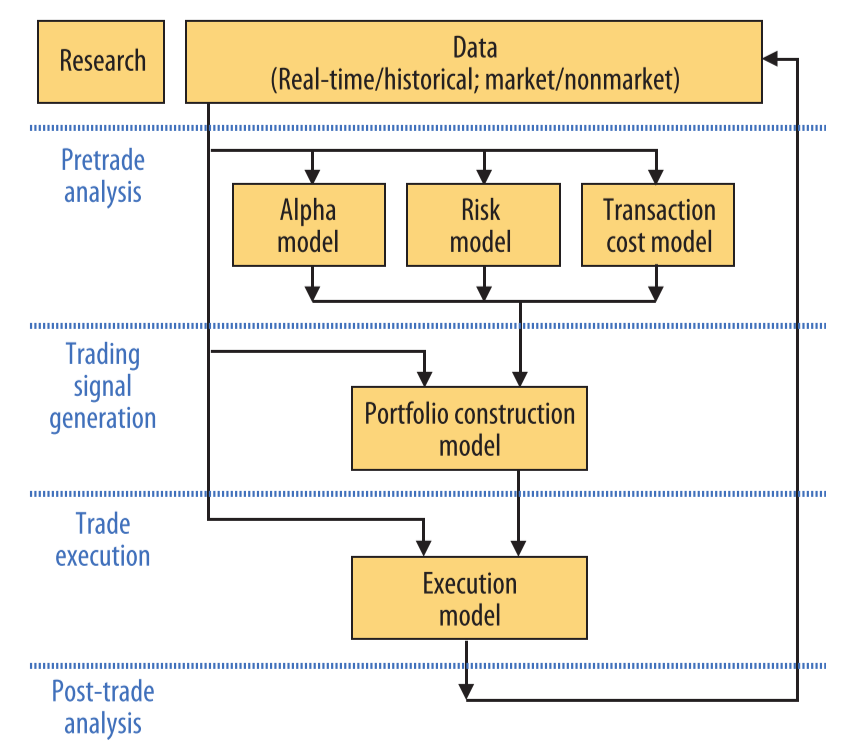
\includegraphics[width=0.55\textwidth]{content/graphics/AT-trade_process}
	\caption{Trade Process Figure by Nuti et al \cite{ART:Nuti:2011}: \textit{(a)} Research / Data, \textit{(b)} Pre-trade Analysis, \textit{(c)} Trading Signal Generation; \textit{(d)} Trade Execution, \textit{(e)} Post-trade Analysis }
	\label{fig:related:tradeprocess}
\end{figure}

Treleaven et al \cite{ART:Treleaven:2013} discuss that access to clean data is crucial to the operation of AT. The specificity of data required depends on the type of algorithm being built. Treleaven et al describe data which can vary from financial, economic, social and news to real-time, historic and analysed market data. The selection and validity of data can greatly affect the operation of AT and requires vetting of cleanliness. This is consistent with Chan's \cite{BOOK:Chan:2013}  discussion of using data to simulate strategies using backtesting, where the results of a strategy may appear positive, but performs poorly when applied to out-sample real-time data. This suggests that the data used in backtesting may be limited, failing to cover the scope of the market. Considering this, implementing a robust system on backtesting that covers various different data sets would ensure that an algorithm can prevent unforeseen issues.

Both Treleaven et al \cite{ART:Treleaven:2013} and Nuti et al \cite{ART:Nuti:2011} describe that pre-trade analysis discerns trading opportunities from data with the aim of predicting future prices to generate trading signals. Specifics of how this is achieved is discussed in section \ref{sec:related:tradingStrategies} (Pg. \pageref{sec:related:tradingStrategies}), but the three main categories of analysis are fundamental\footnote{Information relating to markets to determine an asset's fair value e.g. interest rates}, technical\footnote{Historic, current, and other market information to predict future prices} and quantitative\footnote{Mathematical models based on treating assets prices as random rather than deterministic (like technical analysis)}. As technical analysis is the aim of this project, the forecast of prices and momentum are based on trend indicators and other market data. Three mathematical models: alpha, risk and transaction cost (Fig. \ref{fig:related:tradeprocess}, part b) are used to predict future behaviour, evaluate levels of risk and determine potential costs induced respectively. Each model is crucial to determine the success rate of the entry into - or exit from - the market, but I would emphasise that the risk model may be the most crucial. Taking precautions to ensure risk is minimised is one of the biggest factors to ensure profitable trades, concluded by Engle, Ferstenberg and Russel \cite{ART:Robert:2012} that majority of traders opt for strategies that are risk averse.

Trading signal generation differs from pretrade analysis, specifically determining the values the trade should execute with. Here is why AT positions 90 percent of the daily trade volume \cite{WEB:Cheng:2017,ART:Kolakowski:2018} with its ability to analyse all market information in milliseconds, allowing it to find the entry points with minimal risk. Nuti et al \cite{ART:Nuti:2011} define two problems that could occur during entry, oscillating buy and sell signals and incorrect model assumptions.  Kaufman \cite{BOOK:Kaufman:2013} discusses indicators (Sec. \ref{sec:related:tradingStrategies}, pg. \pageref{sec:related:tradingStrategies}) that can be unprofitable if oscillating prices are failed to be addressed. High transaction costs and increased losses can occur as a result of this. Detecting when to exit by taking profits or minimising losses is crucial, so by failing to address both of these points could lead to an unprofitable and useless signal. 


Finally, Nuti et al \cite{ART:Nuti:2011} and Treleaven et al \cite{ART:Treleaven:2013} states that trade execution determines the constraints a transaction can occur, such as costs or duration. The main point made at this stage is to not adversely affect the market with large orders, while executing trades with reduced risk. Deciding whether to split large orders up into smaller chunks could prevent a change of market momentum, but prolonging the fulfilment of the order could result in failing to obtain the best price. Considering this, research by Engle et al \cite{ART:Robert:2012} states there is a risk component involved in time taken to execute a transaction. The low liquidity and high volatility of the crypto market would bolsters this risk factor, requiring extra attention to trade executions. 


For example, a market order\footnote{Buying/Selling an asset at the best possible price at the current time} during low liquidity would most likely result in overpaying for an asset and increasing volatility, whereas by placing a limit order\footnote{Buying/Selling an asset for a set price} can allow for a better price to fill over a longer period. However, this can also produce issues such as being cut above by a higher placed limit order, reducing the chances of your order filling at the quoted price. Continued analysis even after a trade has executed is required to minimise risk until the order is filled.

The trading process described by Nuti et al \cite{ART:Nuti:2011} and Treleaven et al \cite{ART:Treleaven:2013} correlates with how an algorithmic trading bot to crypto could be implemented. Using the aforementioned process determines steps at the pre-trade analysis stage to minimise risk while considering how to actually execute the trade. Demonstrating research and discussing common pitfalls of these stages shows how a well-designed trading bot can be implemented using technical analysis. While the trade process is discussed, nothing about the actual implementation or success of these systems is mentioned. This paper will discuss how data gathering, pre-trade analysis and signal generation (Fig. \ref{fig:related:tradeprocess}) can be implemented and how signals applied to the nascent crypto market perform, using real data and providing results based on analytics. Although this project looks to build a platform to generate signals on a form of slower pre-trade analysis, High-Frequency Trading constitutes the bulk of AT used in the stock market today. 

\subsection{High Frequency Trading}
\label{sec:related:algoTrading:HFT}
\noindent  Seth \cite{WEB:SETH:0001} states the largest category of the AT cohort is associated to High-Frequency Trading (hereafter, referred to as HFT). While low-latency HFT is not possible in the crypto market (Sec. \ref{sec:related:cryptoAndTheirMarkets}, pg. \pageref{sec:related:cryptoAndTheirMarkets}) - and not used in the development of this project - discussing the effects that HFT has on the stock market is beneficial to evaluating its health and what the crypto market can expect. HFT is the primary trading type in the modern stock market characterised by the speed and volume of trades it can execute within a small-time frame.

Both Seth \cite{WEB:SETH:0001} and Chorida, Goyal, Lehmann and Saar \cite{REPORT:ChordiaEtAl:2013} state the fundamental requirement for a successful HFT algorithm is low-latency - defined by Chorida et al as "strategies that respond to market events in the millisecond environment". This is evident by trading firms spending substantial amounts to be placed as close as possible to the exchange's server to remove milliseconds off latency times \cite{ART:Aswani:2016}. This allows trading firms to respond to the most recent market data, providing the advantage to the first trader that receives the data. Comparing human ability to analyse and respond in this time-frame displays why HFT is the primary method to transact on the market.

Chorida et al \cite{REPORT:ChordiaEtAl:2013} state that most of the liquidity in the stock market is provided by HFT algorithms based on their identifiable activities. This appears inline with an article by Warmbrodt \cite{ART:Warmbrodt:2016}, however he hinges on this as a defence traders use towards the uncertainty regulators face with volatility from events like the 2010 ``flash crash''. He also explains that Clinton had plans for a financial reform to tax certain types of harmful HFT in her presidential race. This reform would of reduced the profitability of HFT, resulting in less firms using this method which may of potentially hindered market quality. Events like the ``flash crash'' shows the extent of controversy that HFT is facing, with Nuti et al \cite{ART:Nuti:2011} and Treleaven et al \cite{ART:Treleaven:2013} basing this on the lack of knowledge towards how they operate. Warmbrodt \cite{ART:Warmbrodt:2016} discusses the findings from an investigation, calling this `predatory' behaviour from aggressive AT firms. 

However, other officials outline the positives of HFT with Warmbrodt \cite{ART:Warmbrodt:2016} quoting the US `Securities and Exchange Commission' (SEC) Chairwoman stating, "[investors] are doing better in today's algorithmic marketplace than they did in the old manual markets". Warmbrodt adds that this is apparent to lower trade costs present in today's markets. The increased liquidity HFT brings allows for larger orders to be successful close to the current price and execute within a short period.  Bajpai \cite{WEB:Bajpai:0001} builds on this by stating that "liquidity is an important characteristic of a good market". The price difference between the highest buy order and the lowest sell order, also known as the `bid-ask spread', reduces transaction costs by producing smaller differences between the buy and sell prices. This incentivises multiple orders to be made consistently by traders, with little transactional cost. In turn, the market is provided with liquidity which ultimately reduces risk for investors. Whether the effects of HFT on the market is resulted by poor understanding or some exploitative behaviour, further research is required to allow regulators to put protective measures in place. 

While Chorida et al \cite{REPORT:ChordiaEtAl:2013} agrees that when HFT operates correctly it can improve the quality of the market with liquidity, it can also degrade it by demanding liquidity without any market makers to fill this demand. This subsequently increases volatility by occurring a major shift in the assets price. Chorida et al state this is evident by the ``flash crash`` of May 2010 where HFT - while it may not of triggered it - certainly affected price volatility. As most HFT algorithms follow trends, they tend to trade on similar rules. An article by Kolakowski \cite{ART:Kolakowski:2018} describes this as `herd' behaviour on steroids, quoting the director of Exchange-Traded Fund (ETF), "when selling happens, more selling can occur and when buying happens, more buying can occur". This can pull liquidity from the market allowing the price to tumble, especially when AT controls roughly \$8.8 trillion according to a 2016 study \cite{ART:Kolakowski:2018}. 

A source from Anagnostidis \cite{UNPUB:Anagnostidis:2017} explains "the speed with which the quotes are posted and cancelled has been criticised by market participants because its creates a false sense of deep liquidity supply for a stock". While this seems to counter previous points of HFT supplying liquidity, it's important to emphasise this is referring to \textit{deep} liquidity. It is undeniable that HFT provides vast amounts of liquidity as mentioned above. Anagnostidis summarises by stating that liquidity generated by submissions and cancellations does not translate into a persistent effect on liquidity supply. This false cushion of liquidity is derived by the current rules followed HFT algorithms and their herd like behaviour as discussed by Kolakowski \cite{ART:Kolakowski:2018}. This can greatly impact the stability of the market as a whole and is the main source for concern about HFT's affect to regulators \cite{WEB:Kaufman:2016}.   

However, this method of `submit-cancel` is also used for price discovery\footnote{Determining price of asset based on analysis of buyer and sellers} of an asset due to AT's precise market analysis. It provides informative predictions based on all market information available leading to readjustment of order prices. An empirical study by Brogaard, Hendershott and Riordan \cite{UNPUB:Brogaard:2017} concluded that HFT improves pricing efficiency\footnote{The assets price is best reflected by all information possessed} by "trading in the price's permanent direction and against transitory pricing errors". This is inline with another empirical study by Benos and Sagade \cite{ART:BENOS:2016} stating non-passive HFT flows in the direction of future price changes. It becomes apparent that price discovery and efficiency is improved by HFT as they tend to follow market trends.  

HFT is possible in the crypto markets but not to the same extent as the equity market. The lack of low-latency connections partially prevents the evident positive and negative effects described above. While tightening spreads, reducing transaction costs, improving price discovery and strengthening price efficiency would contribute to the market's health overall, it is still in an unknown area of regulation to prevent negative damage. This leaves low-latency HFT producing damaging effects with the described `herd' mentality contributing to the rise of flash crashes.  However, with the crypto market still being unregulated with extreme volatility, perhaps employing low-latency HFT could still improve upon the current market's quality. Ultimately, the adverse effects are resulted by the domination of AT in the equity market over many years of development. Perhaps by the time crypto establishes and grows it's market, better regulation for itself and HFT could be further developed.


\newpage
\section{Trading Strategies}
\label{sec:related:tradingStrategies}
\noindent As discussed in the trade process (Sec. \ref{sec:related:algoTrading:tradeprocess}, pg. \pageref{sec:related:algoTrading:tradeprocess}), a well defined trading strategy is the basis of pre-trade analysis. Lien \cite{BOOK:Lien:2016} states that technical analysis works well in the fiat currency\footnote{Legal tender which does not have intrinsic value but declared to have value by the government} market due to its speculative nature and its tendency to overshoot and correct.  Most literature on technical analysis is based on developed equity and currency markets with the discussion on the crypto market being sparse. These handful of related works apply similar indicators that Lien discusses with success, so by evaluating work intended for developed markets will show what trends can be used in the crypto market. This will provide market interpretation for this project and the construction of a sound strategy. I discuss similarities between crypto and other markets in section \ref{sec:related:cryptoAndTheirMarkets} (Pg. \pageref{sec:related:cryptoAndTheirMarkets}).

A paper from Tapa, Yean and Ahmed \cite{ART:Tapa:2016} concluded through their use of moving averages that they were able to return profit on a simple crossover moving average strategy. This single use shows promising results towards the scope of this project, suggesting that technical analysis can be applied effectively to real-time market data. The moving average indicator is one of the most popular identifiers to market momentum by providing clear trends. Kaufman \cite{BOOK:Kaufman:2013}, Lien \cite{BOOK:Lien:2016} and Harmon \cite{BOOK:Harmon:2014} discuss how to apply moving averages and other indicators in practical ways to achieve profitable results. I will also look at the relative strength index (RSI) and moving average convergence/divergence (MACD) momentum indicators and Bollinger Bands (BB) to discuss their beneficial uses toward analysis of market trends.

A moving average (MA) is the mean of closing prices on intervals over a defined period - e.g. 12 days - and is described by Kaufman \cite{BOOK:Kaufman:2013} to remove market noise and find the direction of the price. The most common MA is the simple MA (SMA) which produces an average deduced by all the previous prices with equal weighting. Kaufman \cite{BOOK:Kaufman:2013} states that the SMA can have abrupt changes in value when a significant price movement is dropped off the end due to this equal weighting. This may cause false signals to be generated if recent prices exhibit little change and the older data point had great significance. This could be exceptionally import towards the crypto market due to the extreme volatility they can produce, such as a 15 percent increase in price within a few minutes. 

However, more responsive MAs may suit the crypto market such as the exponential moving average (EMA) suggested by Kaufman \cite{BOOK:Kaufman:2013}, being summarised to give greater weighting to more recent prices. Thus, the effect of dropping off the end price is reduced. This would suggest an improved effectiveness compared to SMA at predicting an accurate trend in the current market price. Harmon \cite{BOOK:Harmon:2014} suggests that using a smaller time-frame with SMA than using an EMA could provide similar results, although, he presents no justification or acknowledgement to the SMA drop-off issue and seems to be merited on opinion. This contrasts with Kaufman's \cite{BOOK:Kaufman:2013} suggestion of using an EMA, however, addresses and expands on this issue with justification. It is worth noting that EMAs are used frequently in other indicators, as I discuss later in this section.
%BOOK Technical Analysis: The Complete Resource for Financial Market Technicians uses Kaufy as a reffy
    
While the SMA can be responsive to the current market price, the weighting of previous prices being equivalent to the current price results in a smooth trend line indicator. Whereas, EMA responds quicker to the current market price, but due to lower weighting of older prices results in a more jagged trend line. I lean more towards EMA to give the best insight towards market trends due to the volatility of crypto's market conditions and hence the need to react to these price changes quickly. However, the use, analysis, and comparison of both MAs in this project will be beneficial to draw conclusions as to which is more effective towards crypto.

Nonetheless, the MA is proven through multiple research papers including Wong, Manzur, and Chew \cite{ART:Wong:2003} who concluded single, dual, and triple MAs produced positive results on the Singapore stock market. They acknowledge that a sideways moving market or times of excessive volatility would generate false signals. Applying the MA by itself to the crypto market may not produce similar results due to its volatile characteristic, so the conjunction of multiple indicators will be required to confirm trends.  

Kaufman \cite{BOOK:Kaufman:2013} describes that the RSI indicates when overbought or oversold conditions occur. This is determined by dividing the total upward price changes over the total downward price changes from a period of time, and then fitted into a range of 0 to 100. This gives the measurement of the current price movement's relative strength over the defined period. This indicator will help determine if a trend reversal is likely to happen based on exceeding or dipping below the threshold values 70 and 30 respectively. Lien \cite{BOOK:Lien:2016} illustrates an example of using RSI to identify when to enter the market. 

\begin{figure}[htb]
    \centering
	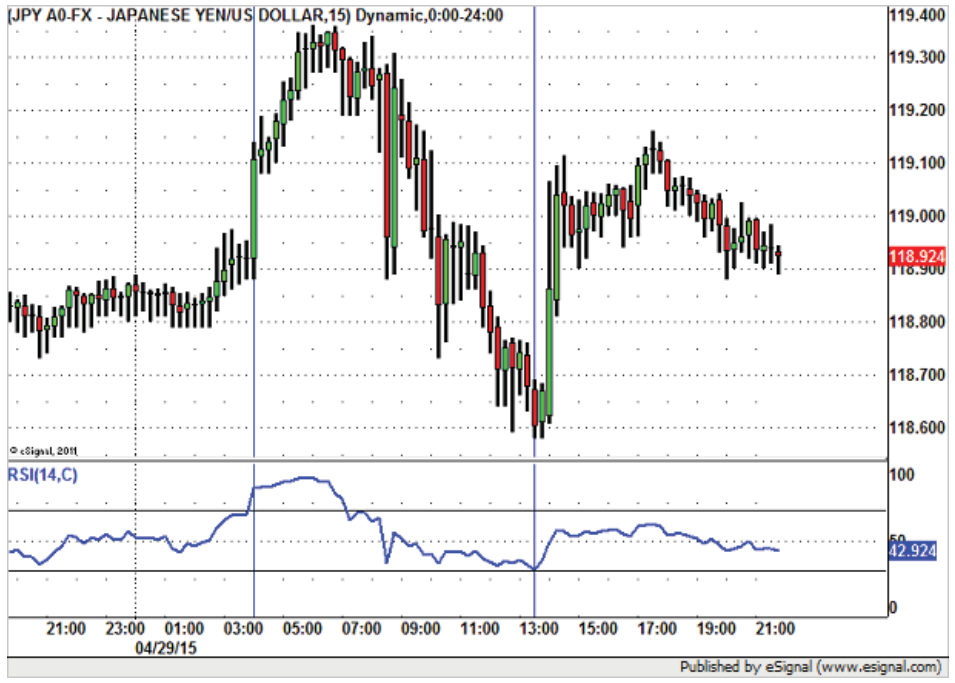
\includegraphics[width=0.7\textwidth]{content/graphics/USDJPY-15_min_chart}
	\caption{USDJPY 15 minute chart by Lien \cite{BOOK:Lien:2016}: \textit{(a)} RSI above 70 at 03:00
	\textit{(b)} RSI at 30 at 13:00}
	\label{fig:related:USDJPY_15min}
\end{figure}

Entering the market at figure \ref{fig:related:USDJPY_15min}.a when the RSI value was above 70 would of seen a market reversal against the entry trade. Waiting until figure \ref{fig:related:USDJPY_15min}.b was the better entry time with the RSI at 30. Although, Kaufman \cite{BOOK:Kaufman:2013} also states that in a study the average amount of RSI values ranges from the 32 to 72 market. He continues, showing that roughly 50 percent of RSI values fall between this range, indicating that the thresholds may need to be widened. Suggestions of 80 to 20 or 85 to 15 are considered extremely strong indicators as they are hard values to sustain. While the example for figure \ref{fig:related:USDJPY_15min} was an ideal scenario, it would be naive to assume this is always the case. Experimenting with threshold ranges to fit this indicator towards the crypto market will be a research point this project looks into.

The MACD is the difference of two EMAs - usually based on 12 (short) and 26 day (long) periods - and another EMA - usually 9 days - that generate trade signals when the lines intersect. Both Harmon \cite{BOOK:Harmon:2014} and Kaufman \cite{BOOK:Kaufman:2013} evaluate the effectiveness of this indicator to be unreliable for trading as it would require the constant fitting of threshold lines to prevent whipsaws\footnote{A volatile price action in which a security swings back and forth in a chaotic pattern}. It would seem that this strategy would work well in an upward or downward market interval, but it would result in poor trades in a sideways market due to whipsaws of the trend line intersections. They state that MACDs are ultimately used to define divergence signals.

Utilising both RSI and MACD in this project's trading strategy will indicate if market reversals are likely to occur or if momentum is still heading in a certain direction. A point Lien \cite{BOOK:Lien:2016} emphasises is the importance of utilising multiple time frames with these indicators as to understand the bigger picture of the market. Failing to analyse where the current moment in the market is can lead to poor trades on the larger scale. Both Kaufman \cite{BOOK:Kaufman:2013} and Harmon \cite{BOOK:Harmon:2014} also discuss this point and conclude that analysis of multiple time frames is important to clarify the current direction of the market.

Another trend indicator which defines oversold or overbought market conditions is the Bollinger Band (BB). It is constructed with three MAs usually based on a 20-day SMA with similar upper and lower bands. The bands are created by adding or deducting the double of the standard deviation of the price over a 20-day period.  Harmon \cite{BOOK:Harmon:2014} analyses the BB to indicate extreme or slight volatility in the price of stocks, discussing when the BB `squeezes' - the upper and lower bands narrow - that volatility has moved out of the stock, indicating a significant price movement is about to occur. 

Harmon \cite{BOOK:Harmon:2014} explains that the price breaking through the upper or lower band indicates an overbought or oversold signal. He states it can be then be used for a trade a signal when the price closes under/above the upper/lower band, confirming a reversal in the trend. This is similar to a strategy Kaufman \cite{BOOK:Kaufman:2013} describes, however he states that the characteristic of a price closing above the upper band ensues a continued trend in an upward trajectory for a few days. This is not conveyed by Harmon \cite{BOOK:Harmon:2014} as he explains the reversal follows shortly after the break through. 

An example of Kaufman's strategy seen in figure \ref{fig:related:BB_trade_strat} would illicit a buy signal when the price closes above the upper band and longing for a period, then shorting when the price closes below the lower band. If the price closes below the middle MA while still longing, the position is closed out as a price reversal is likely, which fits to Harmon's \cite{BOOK:Harmon:2014} strategy but is used to minimise risk rather than a trading rule.

\begin{figure}[htb]
    \centering
	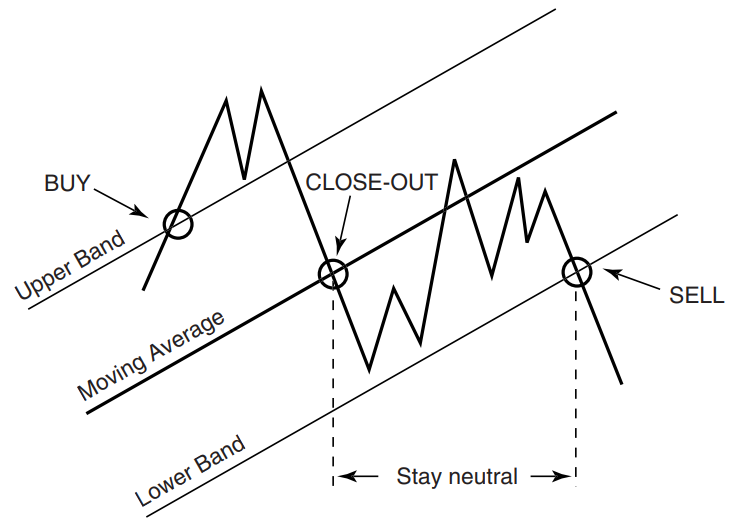
\includegraphics[width=0.6\textwidth]{content/graphics/BB_Trade_Strat}
	\caption{Bollinger Band Trade Signals by Kaufman \cite{BOOK:Kaufman:2013}: 
	\textit{(a)} Buy when price closes above Upper Band
	\textit{(b)} Close position when still longing and price closes below MA
    \textit{(c)} Sell when price closes above Lower Band when shorting}
	\label{fig:related:BB_trade_strat}
\end{figure}

Conversely, the described method by Harmon \cite{BOOK:Harmon:2014} and Kaufman \cite{BOOK:Kaufman:2013} is discouraged by Lien \cite{BOOK:Lien:2016} who explains it's too risky and that two BBs would produce a better strategy. This is the addition of another upper and lower SMA using only the standard deviation of the price. The general rule of thumb is to buy when a trade closes above the first upper band and sell when it trades below the first lower band. Lien describes that while this may not pick the `perfect' bottom, it can avoid a premature entry into an asset. The heightened precautions of the double BB would ultimately minimise risk when using BBs for trade signal generation. Kaufman \cite{BOOK:Kaufman:2013} notes the high risk involved with the trading strategy based on the single BB, strengthening Lien's criticism of this strategy.

Furthermore, Lien \cite{BOOK:Lien:2016} discusses the use of the double BB to indicate when a currency is trending or ranging\footnote{When a price is osculating between similar prices and heading in no clear direction}. This allows to clearly identify the current movements of the market, aiding in the generation of a trading signal. Ultimately, the point of minimised risk deduced from Lien would indicate towards a safer trading strategy while providing clear interpretations of the market. 

The discussion by Kaufman \cite{BOOK:Kaufman:2013}, Harmon \cite{BOOK:Harmon:2014} and Lien \cite{BOOK:Lien:2016} identify trading strategies through the trend indicators described above. Most of the indicators are based on variations of the MA which interprets clear trends the market is currently in. The described indicators, while only capturing the basics of technical analysis, will satisfy the scope of this dissertation by providing clear trade signal generation. While certain strategies can be executed with one indicator, a common point emphasised is the use of a variety of different indicators. Multiple indicators confirming the same trends would provide a stronger signal generation than an individual signal. 


\section{Cryptocurrencies \& Their Markets}
\label{sec:related:cryptoAndTheirMarkets}
% Talk about crypto responding to news and biased trading
% Crpyto is in between currency and securities like stocks, discuss this

\noindent The first cryptocurrency, Bitcoin, made its debut in 2009 with the release of its code base and white paper. This sparked the cryptocurrency market into life which peaked at roughly \$800 billion during its peak in early 2018. It has been reported that the crypto bubble has burst with the current market cap now shy of \$200 billion at the time of writing. Others claim this is just the beginning of a digital currency revolution with the market cap vastly distant from the dot-com bubble where internet stocks were valued at several trillion dollars \cite{ART:Kharpal:2018}. The unpredictability towards crypto's future is attributed by it's uncertainty towards regulation and where it fits into the existing markets. By evaluating this unique market, I can determine if it is profitable, what levels of risk are present and what crypto characteristics to avoid.

From the start of 2017, Bitcoin was worth around \$720. By December it had increased 1,332\% to a peak worth of \$19,783.21 \cite{ART:ELLIS:2018}. This level of movement is unheard of in the equity or currency market, emphasising the extreme volatility of crypto. Last years bull run can be construed as a sudden rush of excitement for the market, which died off after, what Ellis and Swanson \cite{ART:ELLIS:2018} describe as, the price plummeting 66\% (\$6,436). In recent months multiple attempts of reviving the market has taken place by enticing regulation such as multiple Bitcoin ETF proposals to introduce it onto the equity market. The SEC rejected 9 of these proposals which Swanson \cite{ART:ELLIS:2018} claims is due to the concern of lack of transparency and protection for investors. He also mentions that the SEC has concerns of bots manipulating the prices and that exchanges are vulnerable to this manipulation. These are valid concerns as to why Bitcoin is not ready for the equity market, with no protection against volatile price swings and high levels of risk for investors. This ultimately prevents institutional money entering the market and providing stability. 

Vigna and Osipovich \cite{ART:VIGNA:2018} build on this argument stating that some bots are using manipulative `spoofing' strategies. This was outlawed in the US in 2010 but is currently being used to abuse the crypto market. They base this argument around exchanges failing to implement counter measures towards these price jumps, stating "when any venue tolerates manipulative or abusive conduct, the integrity of the entire market is at risk." This ties in with Ellis and Swanson's article \cite{ART:ELLIS:2018} on the SEC's concern towards protection against this market if exchanges are allowing this abuse. 

Other abusive behaviour towards the market can be seen in similar `pump and dump' schemes which Vigna and Osipovich \cite{ART:VIGNA:2018} state generated `\$825 million' over a six month period. This is when a large group of users target a coin, buy a vast portion of the order book and send the price shooting upwards. Then shortly after, they sell at the new high causing the price to plummet while gaining a huge profit. While the market remains unregulated, abusive bots and schemes will exploit it using illegal activities. The effects of these behaviours leaves other traders at a high level of risk, and effects the markets health as a whole.

This is vastly different from regulated markets which monitor for illegal activities \cite{ART:VIGNA:2018}, protecting traders from drastic turns in the market. This attracts large trading institutions to a market with low risk and is why they are avoiding the crypto market. A report by RBC venture capital predicts the crypto market could be worth `\$15 trillion' within 15 years, however it has to first over come risks towards investors. This is why some exchanges are heading down a self-regulatory path, as discussed by Wolfson \cite{ART:WOLFSON:2018}, referring to the Bakkt\footnote{https://www.bakkt.com/} exchange which is in development by Intercontinental Exchange\footnote{https://www.intercontinentalexchange.com/}. This company spawned the New York Stock Exchange (NYSE) and has the infrastructure and experience to bring institutional money with its release. This will bring crypto closer towards regulation, filtering abusive strategies from the market and providing stability.

However, while these developments bring promise they are still a ways off from helping today's market. Swanson \cite{ART:ELLIS:2018} states that big countries are still trying to understand how to properly classify crypto, whether it is a commodity, currency or security. This is due to the multitude of use cases these coins are used for. Some coins are tied to physical assets like oil (Venezeula's Petro Crypto) which, Wolfson \cite{ART:WOLFSON:2018} states bring adherent value and hence liquidity and stability. Other coins are backed one-to-one to a fiat currency (USDT Crypto), and are noted as stable coins due to having this tied value. Some coins are used as utility tokens (IOTA Crypto), to be spent in transactions such as communicating with the Internet of Things (IOT). This conclusively means that different types of coins are valued by different fundamentals and so cannot fit into one specific classification or can necessarily be traded in the same way. An article by Pisani \cite{ART:PISANI:2018} reports a source from the SEC states that Bitcoin is not a security because of its key characteristic of decentralisation. As there is no party that can control it, there is no protection of the asset.

All the aforementioned points will require detailed levels of risk evaluation while stepping through the trade process (Sec. \ref{sec:related:algoTrading:tradeprocess}, pg. \pageref{sec:related:algoTrading:tradeprocess}). Understanding why volatility is so apparent in this market can prepare for the development of this project by being wary of these abusive techniques. Although, as these abusive techniques may look negative towards a regulatory stand point, they don't reflect the profitability that the crypto market holds. Research cited in section \ref{sec:related:tradingStrategies} (Pg. \pageref{sec:related:tradingStrategies}) shows that technical analysis can be applied to the crypto market effectively. Pump and dump schemes discussed by Vigna and Osipovich \cite{ART:VIGNA:2018} mostly target low-cap coins as their prices can be moved with relative ease. They rarely target high-cap coins like Bitcoin as they would require a lot of money to move it. A simple resolution to avoid encountering this type of abusive behaviour is to select specific coins that have a high level of liquidity, high trading volumes, and high market caps. As the time of writing, Bitcoin, Ripple and Ethereum are the top three market caps at \$92, \$19, and \$16 billion\footnote{Taken from https://coinmarketcap.com/}.  


As discussed in section \ref{sec:related:algoTrading:HFT} (Pg. \pageref{sec:related:algoTrading:HFT}), Chorida et al \cite{REPORT:ChordiaEtAl:2013} state low-latency millisecond transactions are essential to the stock market. However, this is not the case for the crypto market due to the inadequate latency times and heavy network restrictions set by crypto exchanges. Bloomberg's Levine reports \cite{WEB:Levine:2018} that only recently updates coming from the largest US based crypto exchange - Coinbase\footnote{https://www.coinbase.com/} - are betting on becoming the first to support low-latency HFT by offering colocation\footnote{Locating computers owned by trading firms inside the same area as the exchange's servers}. This scarcity of low-latency communication between exchange and trader pushes institutional investment further from the market as they can't utilise their trading methods fully.

An article by Meyer and Rennison \cite{ART:Meyer:2017} state that large proprietary HFT firms DRW, Jump Trading, DV Trading and Hehmeyer Trading have entered the crypto market. It would be clear to assume that DRW and others have only entered this space if there is profit to be made. This is due to some HFT strategies not requiring transactions to occur on the millisecond time frame. This suggests that low-latency is not a fundamental requirement for HFT to be successful in the crypto market and the use of other strategies can also be utilised. Literature on algorithms applying technical analysis to the crypto market are sparse, however technical analysis can be applied towards the market successfully as discussed in section \ref{sec:related:tradingStrategies} (Pg. \pageref{sec:related:tradingStrategies}).


It is a common theme from these articles that a full institutional entrance into the crypto market is still a long way off and that regulators are unsure of how to tackle it. With the lack of regulation, avoidance from most institutions and poor infrastructure ultimately marks the crypto market as being a volatile and manipulated entity. However, this does not mean that the crypto market is unprofitable, which Dyhrberg, Foley and Svec \cite{ART:Dyhrberg:2018} conclude in a study that, specifically Bitcoin, has low trading costs and narrower spreads than major equity markets and declare that Bitcoin is investible. Tying this with other aforementioned points, eludes to the careful selection of the coin to be traded on is critical. With this, it is conclusive to avoid low market cap, low volume and illiquid coins. 

\section{Development Libraries \& Web Technologies}
\label{sec:related:developmentLibraries}

\noindent Python is the development language for this project due to its simple syntax and vast number of powerful libraries. The project looks to analyse large quantities of data and make decisions based on this analysis quickly. This requires the use of a fast data structures and analysis which can be fulfilled by the \textit{pandas} \cite{WEB:PANDAS} library. The back testing of the implemented strategies is also a fundamental step of testing as discussed in section \ref{sec:related:tradingStrategies} (Pg. \pageref{sec:related:tradingStrategies}). The library \textit{Backtrader} \cite{MISC:BACKTRADER} can fulfil this requirement. As this project ultimately looks to build a signal generator web app, basic server side implementation is a requirement. Thus, \textit{flask}\footnote{http://flask.pocoo.org/}  will be used to implement a API and WebSocket web server to interact with. Finally, the data used in the project will be provided by the Binance API \cite{WEB:BINANCE_API:2018}. The \textit{Python-Binance} wrapper by McHardy \cite{MISC:Python-Binance} will be used to handle the communications between the bot and their servers as the wrapper has been approved by Binance.

The \textit{pandas} library is listed to deliver "high-performance, easy-to-use data structures and data analysis tools" \cite{WEB:PANDAS}. It consists of two main data structures, Series and DataFrame, with easy selection, merging, computation and date/time series functionality. This library is described by Li \cite{ART:LI:2018} to be "one of the most popular tools for trading strategy development". He explains how stock data can be imported into the DataFrame structure and automatically parsed to be mutable (App. \ref{sec:appendix:code_snippets}, code snippet \ref{code:rel:dev_lib:pandas:amz_data}). One line of code can read external data, parse it and place it into \textit{pandas'} highly changeable and powerful structure. Their documentation is concise, up-to-date, and rich in detail.

The \textit{Backtrader} \cite{MISC:BACKTRADER} library is ultimately used to back-test trading strategies (Sec. \ref{sec:related:tradingStrategies}, pg. \pageref{sec:related:tradingStrategies}) on historical data. The library summarises itself to save time on building code infrastructure and start building trading strategies off of their customisable indicators. They advertise a vast range of coding features to ensure development is simple, such as familiar constructs to get the difference between two MAs (App. \ref{sec:appendix:code_snippets}, code snippet \ref{code:rel:dev_lib:backtrader:sma_diff}). There is support for multiple other built-in indicators such as the BB, RSI, MACD and EMA that is discussed in section \ref{sec:related:tradingStrategies} (Pg. \pageref{sec:related:tradingStrategies}). There is also integrated support with \textit{pandas}. This allows for the combination of both libraries to work seamlessly with each other, avoiding incompatibility issues. This library addresses Chan's \cite{BOOK:Chan:2013} (Sec. \ref{sec:related:algoTrading:tradeprocess}, pg. \pageref{sec:related:algoTrading:tradeprocess}) point on backtesting to ensure a strategy will work with a wide range of in-sample data.

\textit{Flask} is a micro-framework for Python in the use of web development \cite{MISC:FLASK}. As the ultimate goal of this project is to develop a web app, basic web development structures should be considered. However, for the scope of the dissertation, \textit{Flask} will be mostly utilised for a RESTful API and WebSocket integration to the bot and provide modularity so the project can ultimately be tied in with a front-end. These two web technologies provide two different approaches of communicating data, where RESTful API's offer common HTTP functionality such as \textbf{GET} and \textbf{POST} requests and WebSockets provide rooms and namespaces for two way communications.

The \textit{Flask} extension named \textit{Flask-RESTful} provides a lightweight implementation of a RESTful API setup. There documentation demonstrates the minimal code required to prepare specific routes to interact with the server at appendix \ref{sec:appendix:code_snippets}, code snippet \ref{code:rel:dev_lib:flask:flask_restful} (Pg. \pageref{code:rel:dev_lib:flask:flask_restful}). As \textit{Flask} is a framework, there is support for multiple other extensions such as \textit{Flask-SocketIO} that provides WebSocket implementation similar to \textit{Flask-RESTful}. A minimal code example is demonstrated at appendix \ref{sec:appendix:code_snippets}, code snippet \ref{code:rel:dev_lib:flask:flask_socketio} (Pg. \pageref{code:rel:dev_lib:flask:flask_socketio}). Thus, developing the web server integration should be minimal, straightforward, and integrate without complication. As McHardy \cite{MISC:Python-Binance} implements a python-wrapper to communicate with the Binance exchange's API \cite{WEB:BINANCE_API:2018}, the streaming of specific coin pairs (e.g. BTC / USDT\footnote{This represents Bitcoin traded against USDT}) market data, their intervals, and a multitude of other options are easily configurable.  


\section{Conclusion}
\label{sec:related:conclusion}


\noindent Set out by the project's aims, research on relevant literature review of AT (Pg. \pageref{sec:related:algoTrading}), the equity, currency and crypto (Pg. \pageref{sec:related:cryptoAndTheirMarkets}) market, technical indicators that identify market trends (Pg. \pageref{sec:related:tradingStrategies}), and the relevant development libraries and web technologies  (Pg. \pageref{sec:related:developmentLibraries}) have been presented. 

Based on this research, a web app can be developed while considering the difficulties that the crypto market produces. Discussing Treleaven et al \cite{ART:Treleaven:2013} and Nuti et al's \cite{ART:Nuti:2011} in depth analysis of the trade process (Sec. \ref{sec:related:algoTrading:tradeprocess}, pg. \pageref{sec:related:algoTrading:tradeprocess}) prepares the core fundamentals required to implement an AT signal generator. Establishing the point of using reliable, coherent data ensures that the bot can base decisions on trusted sources. This ties together with Chan's \cite{BOOK:Chan:2013} discussion that whole data is required to apply strategies effectively to the real-time market. This is reflected in our preparation of libraries for this project, where \textit{Backtrader} (Pg. \pageref{sec:related:developmentLibraries}) provides a resolution to this concern. 

Furthermore, the evaluation of trend indicators prepares this project with the knowledge of how to analyse the market. This is crucial to developing the basics of an AT bot, which can be fitted towards the crypto market by the evaluation of the crypto market itself. Understanding it's current place in the regulatory area provides clarity to what market this project is dealing with. Discussing  low-latency HFT and its scarcity in the crypto market justifies the development of a TA trading bot, while showing comprehension towards - and awareness to - the future of the crypto market.

Future areas of study should analyse the difference of applying TA between equity markets and the crypto market. This can outline the main differences between the markets to inform future researchers who are approaching developments of similar projects. With more work being applied to the crypto market, the development of its the legal standpoint can be addressed as awareness of this upcoming area grows.




 % INCLUDE: related work
% !TEX root = ../thesis-example.tex
%
\chapter{Requirements}
\label{sec:requirements}

\cleanchapterquote{Innovation distinguishes between a leader and a follower.}{Steve Jobs}{(CEO Apple Inc.)}

\Blindtext[2][1]

\section{System Section 1}
\label{sec:requirements:sec1}

\Blindtext[1][2]

\begin{figure}[htb]
	
\includegraphics[width=\textwidth]{gfx/Clean-Thesis-Figure}
	\caption{Figure example: \textit{(a)} example part one, \textit{(c)} example part two; \textit{(c)} example part three}
	\label{fig:requirements:example1}
\end{figure}

\Blindtext[1][2]

\section{System Section 2}
\label{sec:requirements:sec2}

\Blindtext[1][2]

\begin{figure}[htb]
	
\includegraphics[width=\textwidth]{gfx/Clean-Thesis-Figure}
	\caption{Another Figure example: \textit{(a)} example part one, \textit{(c)} example part two; \textit{(c)} example part three}
	\label{fig:requirements:example2}
\end{figure}

\Blindtext[2][2]

\section{System Section 3}
\label{sec:requirements:sec3}

\Blindtext[4][2]

\section{Conclusion}
\label{sec:requirements:conclusion}

\Blindtext[2][1]
 % INCLUDE: system
% !TEX root = ../thesis-example.tex
%
\chapter{Design}
\label{sec:design}

\cleanchapterquote{You can’t do better design with a computer, but you can speed up your work enormously.}{Wim Crouwel}{(Graphic designer and typographer)}

\Blindtext[2][2]

\section{Postcards: My Address}
\label{sec:design:address}

\textbf{Ricardo Langner} \\
Alfred-Schrapel-Str. 7 \\
01307 Dresden \\
Germany


\section{Motivation and Problem Statement}
\label{sec:design:motivation}

\Blindtext[3][1] \cite{Jurgens:2000,Jurgens:1995,Miede:2011,Kohm:2011,Apple:keynote:2010,Apple:numbers:2010,Apple:pages:2010}

\section{Results}
\label{sec:design:results}

\Blindtext[1][2]

\subsection{Some References}
\label{sec:design:results:refs}
\cite{WEB:GNU:GPL:2010,WEB:Miede:2011}

\section{Make Something Here}
\label{sec:design:CHANGEME}
 % INCLUDE: design
% !TEX root = ../thesis-example.tex
%
\chapter{Evaluation}
\label{sec:evaluation}

The evaluation of this project was split into three categories. A system usability evaluation of the web app was conducted to gather data on it's intuitiveness and ease of use, a testing suite was created to evaluate robustness of the web server and it's responses when operating the bot and platform and an empirical study of different strategies and their parameters to provide comparisons on their performances. These categories cover all parts of development of this project and evaluate them appropriately.


\section{Web App Usability}
\label{sec:evaluation:ui}
\noindent The purpose of the system usability evaluation aims to identify if the web app is intuitive for new and experienced users to the cryptocurrency market and evaluates the implementation of the front end (Sec. \ref{sec:implementation:frontend}, pg. \pageref{sec:implementation:frontend}). The candidates level of knowledge on cryptocurrencies and their experience of using cryptocurrency or stock markets was recorded to identify how the web app is used with these different levels of experience, and what issues the candidates faced. The evaluation required the candidate to complete tasks using the web app and to provide feedback and rate the tasks while being observed. The tasks tested how the web app presents,
\begin{enumerate}
\item Coin pair information
\item Controls for the bot
\item Trade signals 
\item Strategy configurations
\item Feedback on operations executed by the bot
\item Selection of different coin pairs
\item Live market depth
\end{enumerate}

% TASK 1 IN EVAL

\noindent To analyse how the web app presents coin pair information, candidates were tasked with gathering information about what coin pair was currently selected, the last traded price, the highest and lowest 24 hour price and the total volume traded in 24 hours. My initial hypothesis for completing this task was to be relatively straightforward as all this information is contained at the top of the web app. While this was partially true, this result mainly came from users who state they had atleast some experience using a cryptocurrency exchange. One candidate stated, "All the data was available on the top of the screen where your eyes naturally look for the information if you have used any form of stock trading." Another states, "Naturally, I looked at the top of the screen as that is where a price ticker tends to be on a cryptocurrency exchange."

However, some candidates who have only heard of cryptocurrency exchanges but have never used one struggled with this. One candidate tried to find this data within the candlestick chart and coin pair listings, which does display relevant data, but not clearly or easily. This candidate did complete the task after noticing the top bar but stated "I am new to trading platforms, the GUI [\textit{appears to be}] busy and can be overwhelming. However, after a few minutes, you begin to get a feel for it and know what each section represents." 

% TODO may need updated with more candidates, maybe charts as well?
Candidates could rate this task between 1 (Very difficult) and 5 (Very easy), where most rated it at a 5. This shows this design is intuitive and familiar with most candidates and suggests that understanding how to derive specific data from the panels is straightforward. Although, for inexperienced users, the initial learning curve looks to be the biggest issue with the lowest rating rated at a 2. This seems to persist as a repeating issue throughout this evaluation.

From this first task, a clear distinction in knowledge attributes to the different approaches of completing it. Inexperienced users felt lost and overwhelmed within the UI and struggled to derive data displayed at the top of the page initially, whereas experienced users spotted this panel straightaway. A future solution to solve this issue may be to introduce a \textit{one-time pop up}. This pop up would occur on a users first visit to the page and present a quick description over each section of the UI. This would give the user a basic knowledge of what information the user is presented with and how to understand it as to allow them to be familiar with the web app as quick as possible.

% TASK 2 AND 4 IN EVAL
\noindent Candidates were tasked to start the bot and then stop the bot in a later task. These tasks were issued separately and non-sequentially as they both require a similar approach to completing them. This can bring a measure to how candidates approach the web app as they become more familiar with it. All candidates found the button easy to identify when trying to locate it to start and stop the bot.

Candidates were also requested to provide feedback about how they could confirm the bot had successfully completed this operation and if they felt informed about what the bot's current status was. Most candidates found that the snackbar (pop-up) notification was helpful in confirming the bot had completed the operation and that it was not intrusive on the web app. Some candidates noted on the button being a toggle for the operations and that it was "natural to click it again to turn it off". This provides clear testimonials that basic bot operations are concise and natural for a user to understand.

After completing each task, candidates were asked to rate how clearly they were informed of the bots status on a scale between 1 (Very unclear) and 5 (Very clear). Most rated 5, stating that they were informed very clearly. However, one candidate, who describes themselves as spending a lot of time using cryptocurrency exchanges, rated 3 on the first task. On the second task that required the candidate to stop the bot, they increased their rating to a 4. This suggests that after spending time using the web app to complete similar task, a user becomes more familiar with how it operates and feels more informed about what to expect from the web app. This further confirms that their is a learning curve to using the web app and that users can become more familiar with it as they spend time using it.

This outcome is interesting however as this candidate has experience of cryptocurrency exchanges where their likeness pertains to this web app, yet they were one of the only candidates that did not feel they were clearly informed. This candidate left feedback after completing the first task stating, "The indicators don't give a lot of context as to what is happening, it requires some working out to realise that they obviously say \textit{up} and \textit{down}." While the indicators the bot generated on the candlestick chart were not a part of this task, only two candidates - both of whom are experienced with cryptocurrency exchanges - noticed the effect the bot had on the candlestick chart after starting it. The other candidate noted they felt very informed of the bot's current status even after noticing the signal indicators on the candlestick chart, so this may be the result of whether the first candidate felt informed about what the bot had displayed on the candlestick chart rather than what the bot's current status actually was. This will be discussed further in the trade signals discussion below.

A final point to make on these tasks is the little mention of the operational messages panel. No candidate noted on it, favouring to look at the snackbar notification solely. This panel is important for keeping a log of current and past events as to allow a user to stay fully informed of all recent actions. This presents the issue that when important and descriptive notifications are displayed on this panel, they may be overlooked by the snackbar, which by design only highlights a high level overview message. A few solutions to making the push message panel more prominent could be to prevent the snackbar overlapping it, to add a transition animation for when a new message is received and to make it more attractive through colours. 

\noindent 


% Evaluation of the front end implementation will be compared towards the functional requirements \textbf{FR-1, FR-2, FR-3, FR-4, FR-5, FR-6, FR7, and FR-8} in table \ref{table:requirements:func} (Pg. \pageref{table:requirements:func}). As these requirements have been catered towards the aims and objectives, this will validate the completion of the project.


\section{Web Server Testing}
\label{sec:evaluation:web_server}

\noindent An evaluation of the web server's robustness and ability to respond to events is tested through unit tests on all of the available endpoints and can be used to draw conclusions on the implementation of the information and communications process (Sec. \ref{sec:implementation:info_comm}, pg. \pageref{sec:implementation:info_comm}). Specifically, this section looks to evaluate the process performed by the part of the web server that handles the forwarding of data received from Binance to the user. This includes when the 429 status code is received or an API restriction is in affect. Testing of the web server's communication between a user and a bot is also performed by testing if input is validated, if the responses are appropriate for the outcome of the operation and if API restrictions are handled appropriately. There are 10 unit tests in total that cover the exceptions stated above that the web server may encounter during operation, however this is a non-exhaustive list.


\subsection{Exchange Data Endpoints}
\label{sec:evaluation:web_server:exch_data}
% Unit tests on data end points

% TODO update the 'listed requirement'
\noindent Retrieving exchange data from Binance in a controlled and non-abusive manner is one of the listed requirements of this project. This means that the 429 status code that can be received from Binance is required to be handled appropriately through the implemented self-ban functionality. Therefore, the unit tests listed in table \ref{sec:evaluation:web_testing:exch_data:all_tests} have been created to confirm this functionality works robustly. The endpoints listed in table \ref{sec:evaluation:web_testing:data_apis} and \ref{sec:evaluation:web_testing:data_ws} are some of the web server's Binance data endpoints that are tested by the unit tests in table \ref{sec:evaluation:web_testing:exch_data:all_tests} because they perform API requests to Binance. 

\begin{table}[ht]
\centering
  \begin{tabularx}{\linewidth}{|c|c|L|c|} 
    \hline
    \textbf{ID} & \textbf{Endpoint Type} & \textbf{Description of Test} & \textbf{Outcome} \\ 
    \hline\hline
    1  & API & Spam the \textbf{allCurrencyPairs} endpoint until a non-200 request is returned. & Pass    \\ 
    \hline
    2  & API &   Spam the \textbf{orderbook} endpoint until a non-200 request is returned.  & Pass    \\ 
    \hline
    3  & WebSocket & Trigger the \textbf{connect} event of the \textbf{candlestick} endpoint when a self-ban has occurred & Pass    \\ 
    \hline
    4  & WebSocket &  Trigger the \textbf{get\_klines} event of the \textbf{candlestick} endpoint to stream data when a self-ban has occurred. & Pass    \\
    \hline
  \end{tabularx}
\caption{Binance Data Endpoint's Unit Tests and Results}
\label{sec:evaluation:web_testing:exch_data:all_tests}
\end{table}

\noindent Unit tests 1 and 2 in table \ref{sec:evaluation:web_testing:exch_data:all_tests} test the endpoints 1 and 2 in table \ref{sec:evaluation:web_testing:data_apis} respectively. Each endpoint has a fetch request repeatedly sent until a non-200 status code response is returned; due to a 200 status code representing an OK (normal) response. The web server is then expected to return a 429 status code response that is received from Binance to inform the user that the web server is currently restricting API requests. To confirm the self-ban is fully in place, another fetch request is sent immediately after to retrieve data from the endpoint, where another 429 status code is expected to be returned again.

When the 429 status code is ultimately returned to the user who originated the request, it confirms that the web server has appropriately handled the setting or abiding of an API restriction. This is because that, by design of how the web server handles requests, a 429 status code can only be returned from the web server when it has restricted itself from API requests. However, in production this could lead to abuse of the API and ultimately restrict the web server from requesting data entirely. Therefore, a solution for this project could be to either implement an endpoint weighting system similar to the system Binance has, or store local caches of data that are frequently requested to prevent requiring extra calls to their API for the same data another user has requested. 

% TODO maybe compare either solution, does either aid to the objectives or the current project?
While the first party endpoint weighting solution would prevent abuse and lower the chance of requiring self-bans, it would fail to support a large number of concurrent users who would still require requests to gather the data. Implementing this alongside the caching solution would prevent abuse to the web servers endpoint and reduce API calls to Binance as well. This would also further the projects objective of creating a robust web app that can handle varied exception cases.

\begin{table}[ht]
\centering
  \begin{tabularx}{\linewidth}{|c|c|L|} 
 \hline
\textbf{ID} & \textbf{Endpoint URL} & \textbf{Description} \\ 
\hline\hline
1  &   \textbf{allCurrencyPairs} & Returns overview data of all coin pairs.    \\ 
\hline
2  &  \textbf{orderbook@<coin-pair>} & Takes parameter \textit{<coin-pair>} (e.g. `BTCUSDT') and returns current orders in the order book for that coin pair.    \\ 
\hline
\end{tabularx}
\caption{API Endpoints for Binance Data
\textbf{NOTE :} All endpoints are prefixed with \textit{\textbf{"/api/v1/"}}}
\label{sec:evaluation:web_testing:data_apis}
    \end{table}

\noindent Unit tests 3 and 4 in table \ref{sec:evaluation:web_testing:exch_data:all_tests} test the sole WebSocket endpoint that requests data from Binance's API during its events. This occurs during the \textbf{connect} and \textbf{get\_klines} events of the \textbf{kline} namespace (described in table \ref{sec:evaluation:web_testing:data_ws}), therefore a unit test was created for each event. Both events ultimately return a JSON response with the key \textbf{status\_code} that has the value \textbf{429} when it encounters the self-ban restriction. This provides context as to why the operation was unable to complete and provides the interface that uses the endpoint with a way to handle the response appropriately.

The exception responses from the data endpoints currently don't provide any other data other than the keys \textbf{status\_code} and \textbf{msg}. In future works, the web server could return a response to generate a log message, as discussed in section \ref{sec:implementation:frontend:controls_notifications} (Pg. \pageref{sec:implementation:frontend:controls_notifications}), to alert the user that the service is temporarily unavailable. This could also be tied in with the implementation of the web servers own endpoint weighting system to provide updates to the user about any issues the web server is facing or what restrictions are being applied to them. Working examples of this are already implemented in the bot's controller endpoints discussed in section \ref{sec:evaluation:web_server:bot_controls} below.

\begin{table}[ht]
\centering
  \begin{tabularx}{\linewidth}{|c|c|L|} 
    \hline
    \textbf{ID} & \textbf{ \textit{namespace}@\textit{event}} & \textbf{Description} \\ 
    \hline\hline
    1  &   \textbf{kline@connect} & Initial connection to candlestick data's namespace. Performs an API fetch to Binance to confirm its online and serving data. \\ 
    \hline
    2  & \textbf{kline@get\_klines} & Takes coin pair (e.g. BTCUSDT) as data on triggering this event. Performs initial API fetch to Binance for historic data, then creates a WebSocket connection to Binance's WebSocket endpoint and streams the historic and new data back to client who triggered the event. \\ 
    \hline
  \end{tabularx}
\caption{WebSocket Endpoints for Binance Data: 
\textit{(a)} \textbf{\textit{namespace}} is the url for the WebSocket \textbf{NOTE :} All namespaces are prefixed with \textit{\textbf{"/ws/binance/"}}
\textit{(b)} \textbf{\textit{event}} is the event that can be triggered on the namespace to perform a certain action }
\label{sec:evaluation:web_testing:data_ws}
\end{table}

\subsection{Bot Control Endpoints}
\label{sec:evaluation:web_server:bot_controls}
% Unit tests on bot end points

\noindent To ensure robustness of the endpoints that control operations that a user can perform on a bot, a range of test cases are used to test the responses returned by the web server. The test cases listed in table \ref{sec:evaluation:web_testing:bot_controls:all_tests} cover how a bot handles a 429 code that is received from the web server, input validation on data arguments sent to the web server and the normal operations of controlling a bot.

\begin{table}[ht]
\centering
  \begin{tabularx}{\linewidth}{|c|c|L|c|} 
    \hline
    \textbf{ID} & \textbf{Endpoint Type} & \textbf{Description of Test} & \textbf{Outcome} \\ 
    \hline\hline
    1  & API & Start and stop the bot under normal conditions. & Pass    \\ 
    \hline
    2  & API &  Start the bot with missing arguments. & Pass    \\ 
    \hline
    3  & WebSocket & Start the bot under normal conditions. & Pass    \\ 
    \hline
    4  & WebSocket & Start the bot with missing arguments. & Pass    \\ 
    \hline
    5  & WebSocket & Start the bot with no data. & Pass    \\ 
    \hline
    6  & WebSocket & Start the bot with data an API restriction in affect. & Pass    \\ 
    \hline
  \end{tabularx}
\caption{Bot Endpoint Unit Tests and Results}
\label{sec:evaluation:web_testing:bot_controls:all_tests}
\end{table}

Endpoint 1 in table \ref{sec:evaluation:web_testing:bot_apis} and \ref{sec:evaluation:web_testing:bot_ws} interface with the bot in the same way but provide access through two different protocols. While endpoint 1 in table \ref{sec:evaluation:web_testing:bot_apis} is unnecessary for the scope of this project, it is still being discussed and tested here for possible future work. Having this endpoint tested and available allows access from other interfaces that may not support WebSockets but can still communicate through HTTP endpoints. 
\begin{table}[ht]
\centering
  \begin{tabularx}{\linewidth}{|c|c|L|} 
    \hline
    \textbf{ID} & \textbf{Endpoint URL} & \textbf{Description} \\ 
    \hline\hline
    1  &   \textbf{bot/start} & Returns overview data of all coin pairs.    \\ 
    \hline
    2  &  \textbf{bot/stop@<hash-id>} & Takes parameter \textit{<hash-id>} (e.g. "fa25f6...") and returns response appropriate to the outcome of the operation.    \\ 
    \hline
  \end{tabularx}
\caption{API Endpoints for Bot Control 
\textbf{NOTE :} All endpoints are prefixed with \textit{\textbf{"/api/v3/"}}}
\label{sec:evaluation:web_testing:bot_apis}
\end{table}

Unit tests 1 and 3 in table \ref{sec:evaluation:web_testing:bot_controls:all_tests} check whether the bot can start under normal conditions. These tests are useful to confirm if any changes to the project may have affected the start or stop controls of a bot. The initialisation can be executed with the WebSocket or API endpoint, but the WebSocket endpoint is the main endpoint used due to the streaming of signal data to the front end UI. The WebSocket test checks that two JSON responses are received from the server containing the two different message types, as discussed in section \ref{sec:implementation:frontend:controls_notifications} (Pg. \pageref{sec:implementation:frontend:controls_notifications}). 

% TODO add code snippets of expected JSON responses of logs
The log message type holds the import data about the outcome of this endpoint, containing the key \textbf{success} that has the value \textbf{true} when the bot has started, or \textbf{false} if it failed to do so. The bot's unique hash ID is also a part of this response and is confirmed that it has been received while ensuring it is a length of 32 characters. The snackbar message type provides styling information for the pop up message of the frontend by having the key \textbf{variant} with the value \textbf{success}. This provides details about what kind of message the UI should display, in this case a green \textit{success} message.

Unit test 1 in table \ref{sec:evaluation:web_testing:bot_controls:all_tests} is checked for the same data, however only one response is possible and does not have a specific message type. This endpoint is a more direct method to interacting with the bot and its response is not decorated for the front end UI. This endpoint is useful for interfaces that may want to interact with the web server through there own third party service, similar to how this web server interacts with Binance's server. 

Unit test 2 and 4 in table \ref{sec:evaluation:web_testing:bot_controls:all_tests} attempt to the start the bot with missing arguments. The initial testing using test case 4 resulted in the case failing as there was no proper input validation implemented for the WebSocket endpoint, but the API endpoint had built-in functionality to validate its own input. Thus, to ensure consistency with the API when unexpected input was sent to the web server, the WebSocket was re-factored to handle inputs in a similar fashion to the API. This required creating a function to parse the data retrieved and perform basic checks that all the arguments were present. 

Unit test 4 was originally failing as success messages were received, which would be the same results that would pass unit test 3. This obviously would be an incorrect result for when data is missing and therefore it is correct that the test failed. To create a passing result, unit test 4 should require two message types, with the log type returning the key \textbf{success} containing the value \textbf{false} stating the bot failed to start and with the key \textbf{botHash} also containing the value \textbf{none} because the bot did not successfully start. The key \textbf{missing\_args} is also returned with a list of what arguments are missing. This provides an easy way to define what parameters are missing from this endpoint which creates a more maintainable and informative response. 

Unit test 5 in table \ref{sec:evaluation:web_testing:bot_controls:all_tests} attempted to start the bot with no data at all. The re-factor discussed above did not handle data that was fully missing and therefore required the endpoint to be re-factored further. This unit test now expects the key \textbf{success} to be returned with the value \textbf{false} and the key \textbf{msg} to return an appropriate explanation about why the bot failed, which in this case returns, \textbf{"Bot failed to start, no data was received."} This endpoint conforms to an acceptable level of robustness and provides informative data to a bad request. 

Unit test 6 tests a bot that is started through a WebSocket and receives a 429 status code from the web server's candlestick endpoint (2 in table \ref{sec:evaluation:web_testing:data_ws}) for Binance data. The bot would still start as usual and return the same messages that were discussed for unit test 3, but after the bot creates a connection to the candlestick endpoint, three responses are expected to be returned. The first two are the log and snackbar messages to inform the user on the front end that the bot couldn't gather data due to an API restriction and should retry later. The third response is an event call for the front end that triggers the \textbf{stop\_bot} event. This is used to update the UI to inform the user the bot is no longer running. This is important as it allows any interface using the service to handle the event of the server force stopping the bot.

\begin{table}[ht]
\centering
  \begin{tabularx}{\linewidth}{|c|c|L|} 
    \hline
    \textbf{ID} & \textbf{ \textit{namespace}@\textit{event}} & \textbf{Description} \\ 
    \hline\hline
    1  &   \textbf{communicator@bot\_start} & Initial connection to candlestick data's namespace. Performs an API fetch to Binance to confirm its online and serving data. \\ 
    \hline
  \end{tabularx}
\caption{WebSocket Endpoints for Bot Control: 
\textit{(a)} \textbf{\textit{namespace}} is the url for the WebSocket \textbf{NOTE :} All namespaces are prefixed with \textit{\textbf{"/ws/v3/bot/"}}
\textit{(b)} \textbf{\textit{event}} is the event that can be triggered on the namespace to perform a certain action }
\label{sec:evaluation:web_testing:bot_ws}
\end{table}

% \noindent Evaluation of our server infrastructure implementation can be confirmed by our completion of requirements \textbf{NFR-1, NFR-2, NFR-6, and FR-9} in tables \ref{table:requirements:non_func} and \ref{table:requirements:func} (Pg. \pageref{table:requirements:non_func} and \pageref{table:requirements:func}). The analysis undertaken is equivalent to section \ref{sec:evaluation:tradeprocess}.



\section{Strategies Comparison}
\label{sec:evaluation:strats}

\noindent A range of different strategies will be empirically evaluated and compared against one another by analysing their performance such as the amount of signals generated and the final net value. These strategies will be evaluated on the BTC / USDT coin pair. A mock starting balance of 10,000 USDT (1 USDT = 1\$, hereafter USDT will be represented as \$) will be used for each strategy and a commission rate of 0.1\% will occur on each signal to simulate real trades that are subject to trading fees on cryptocurrency exchanges. A trade will buy or sell exactly 1 BTC at the closing price of the interval of the signal to make the comparisons straightforward. This means that if a buy signal is generated at \$4,800 and a sell signal at \$5,000, the total gross amount would be \$200. This would make the initial portfolio value of \$10,000 become the gross amount \$10,200. Then commission will be subtracted from the \$200 trade it to bring a total net amount.

The strategy's generated signal data has been collected from the \textbf{13-03-19} to the \textbf{10-04-19}, which corresponds to one thousand 30 minute intervals. During this period, the BTC / USDT pair had a significant upward movement in price around three quarters of the way through this period with a mostly sideways moving market throughout the other intervals.
 
 \iffalse
\begin{table}[ht]
\centering
  \begin{tabularx}{\linewidth}{|c|L|c|c|c|} 
    \hline
    \textbf{ID} & \textbf{Strategy Name} & \textbf{Signals Generated} & \textbf{Net Portfolio} & \textbf{Net Profit} \\
    \hline\hline
    \textbf{1} & RSI & 2 & 10,062.00 & 62.00 \\
    \hline
    \textbf{2} & MACD & 105 & 10,239.98 & 239.98 \\
    \hline
    \textbf{3} & SMA Crossover & 51 & 10,614.42 & 614.42 \\
    \hline
    \textbf{4} & SMA Crossover \& RSI & 0 & 10,000.00 & 0.00 \\
    \hline
    \textbf{5} & SMA Crossover \& MACD & 47 & 10,550.62 & 550.62 \\
    \hline
    \textbf{6} & Bollinger Bands & 25 & 10,925.39 & 925.39 \\
    \hline
    \textbf{7} & Double Bollinger Bands & 1 & 11,501.65 & 1,501.65 \\
    \hline
  \end{tabularx}
\caption{The total number of signals generated and the net portfolio that is resultant of the default parameters for each strategy. The \textbf{Net} column headers are in USDT.}
\label{sec:evaluation:strats:performance}
\end{table}
\fi

\subsection{RSI Strategy}
\label{sec:evaluation:strats:rsi}

\noindent The performance of the RSI with configuration 1 in table \ref{sec:evaluation:strats:rsi_allvariants} seems to be quite reserved by only generating 2 signals over the month period. The signals for this configuration created the least total profit compared to the other strategies with a total of \$62.00. 

\begin{table}[ht]
\centering
  \begin{tabularx}{\linewidth}{|c|L|L|L|L|L|} 
    \hline
    \textbf{ID} & \textbf{Upper Threshold} & \textbf{Lower Threshold} & \textbf{Signals Generated} & \textbf{Net Profit} \\
    \hline\hline
    \textbf{1} & 70 & 30 & 2 & 62.00 \\
    \hline
    \textbf{2} & 60 & 40 & 26 & 498.00 \\
    \hline
    \textbf{3} & 80 & 20 & 2 & 202.15 \\
    \hline
  \end{tabularx}
\caption{\textbf{RSI} strategy with all configuration variants that were evaluated; ID 1 is the default parameters for this strategy; The {Net} column headers are in USDT.}
\label{sec:evaluation:strats:rsi_allvariants}
\end{table}

Configuration 1's long signal was generated at the price \$3910.00 and the sell signal at \$3972.00, but looking at the candlestick chart at figure \ref{fig:f1} for these signals, they show a concerning price movement. Before the short signal (red downwards arrow), the market dipped drastically; to then only spike and recover.  As the RSI indicator defines overbought or oversold conditions, it fails to react to the market and therefore could easily have resulted in a significant loss of the portfolio. Furthermore, by looking at the candlestick charts in figure \ref{fig:eval:strats:rsi_signals}, they suggest that a market reversal is not 100\% certain due to the chart price progression following the last short signal. The market actually continues to trend upwards for the rest of the month. The strategy may have benefited from smaller thresholds in this specific instance as the whipsaws between these two signals nearly cross the thresholds but fall short.

\begin{figure}[ht]
  \centering
  \subfloat[Upper threshold 70 and lower threshold 30]{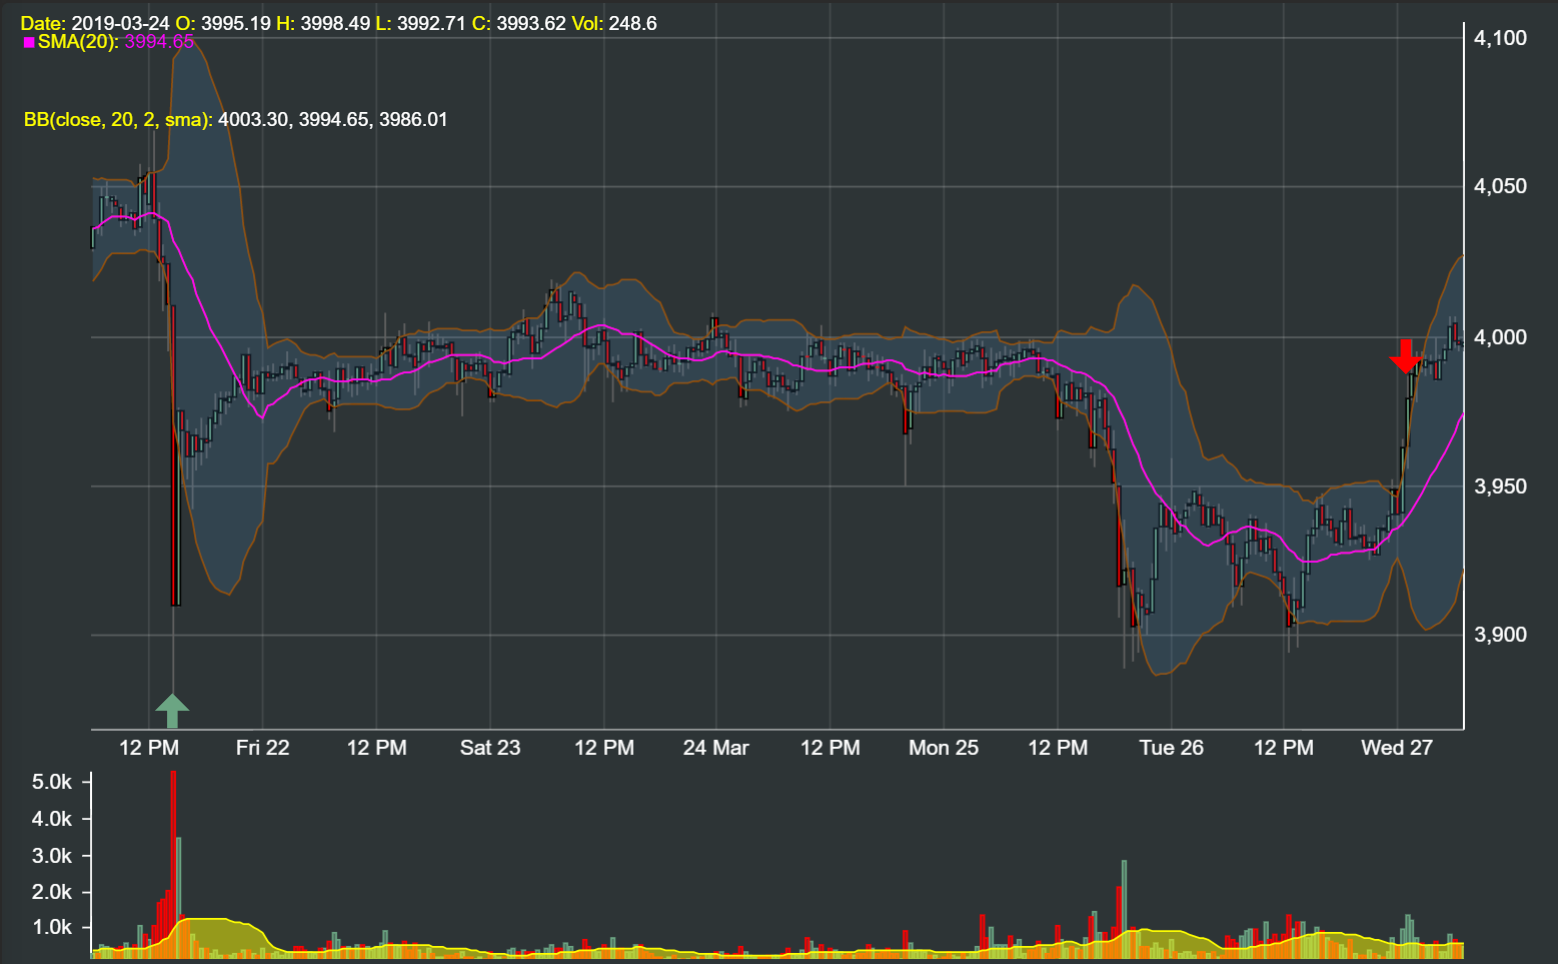
\includegraphics[width=0.495\textwidth]{content/graphics/rsi_default_sg1_sg2.PNG}\label{fig:f1}}
  \hfill
  \subfloat[Upper threshold 60 and lower threshold 40]{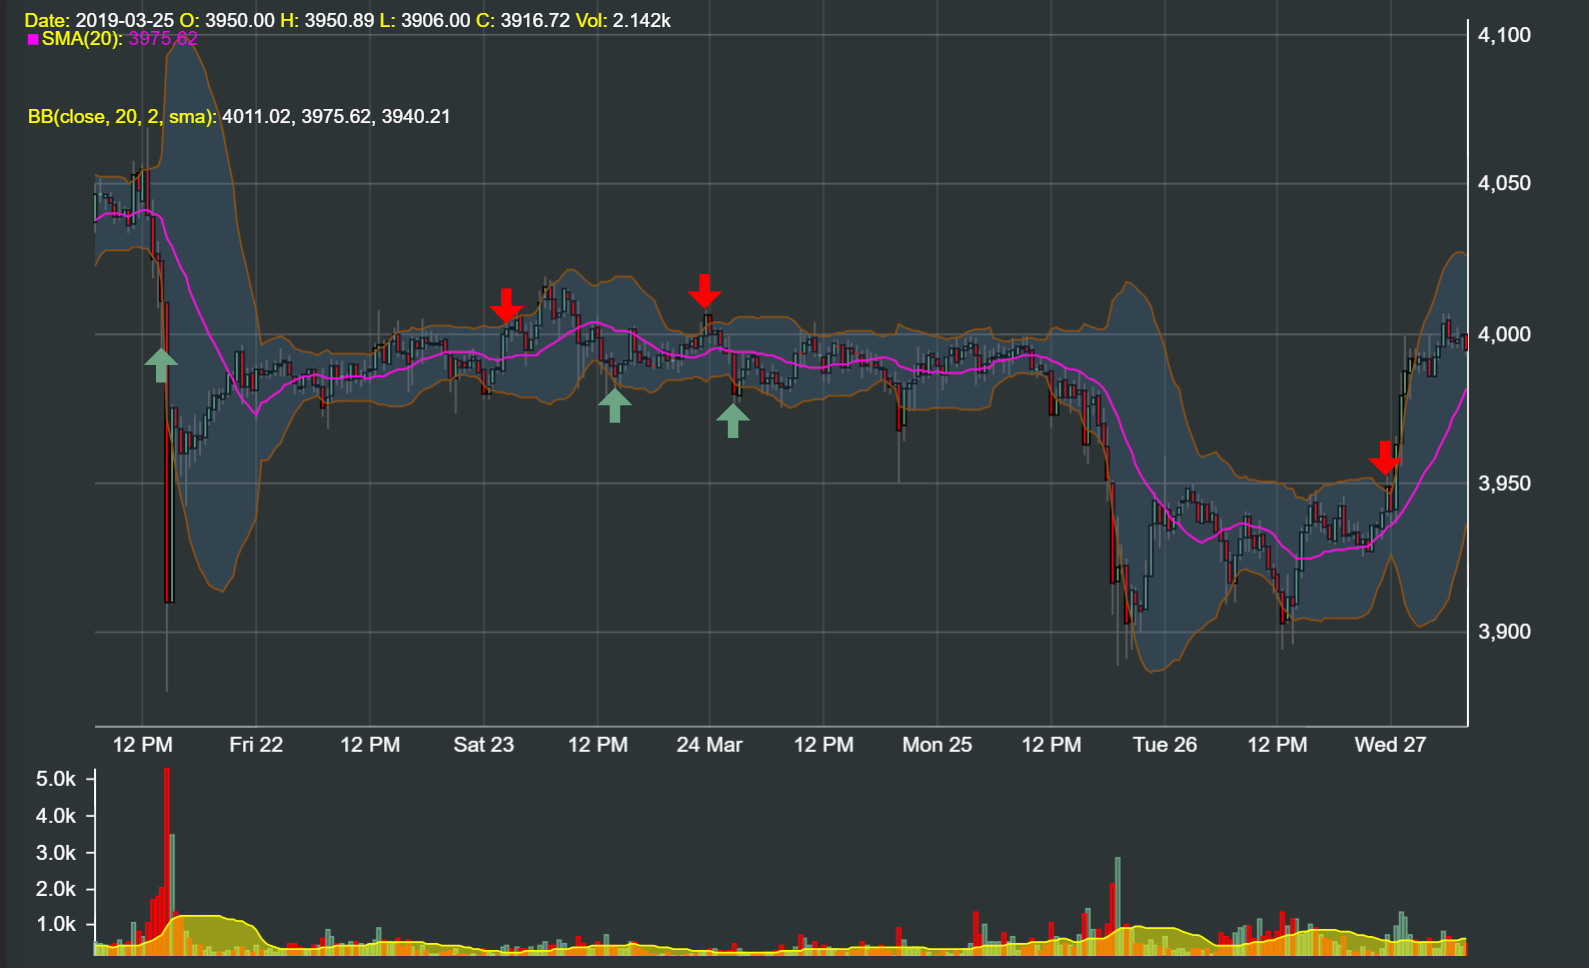
\includegraphics[width=0.5\textwidth]{content/graphics/rsi_60_40_same_period.PNG}\label{fig:f2}}
  \caption{RSI strategy trade signals with different thresholds}
  \label{fig:eval:strats:rsi_signals}
\end{figure}

For configuration 2 in table \ref{sec:evaluation:strats:rsi_allvariants}, the upper and lower thresholds at 60 and 40 respectively, return a more profitable strategy. 26 signals are generated rather than 2, with a net portfolio value of \$10,498.73. This is a significant improvement over the default 70 and 30 values. However, comparing the figure \ref{fig:f2} with fig \ref{fig:f1} which span the same period, it is clear that the strategy doesn't find the lowest price of significant drops. The first long signal in figure \ref{fig:f2} is generated before it reaches the lowest price. Although, it does manage to generate the signals within the whipsaws, the lower thresholds still fail to react to the sudden drop off before the last shown signal.

It could be argued that the thresholds at 60 and 40 produce less risk as they generate signals between smaller price ranges. This means that the larger price difference displayed at the 70 and 30 threshold chart would be less likely to occur, reducing the amount of assets being traded at once. Lots of smaller trades also add up as evident by the greater profit gain from the parameters of this strategy. This strategy with the 60 and 40 parameters is still far from perfect however, as the indicators prematurely enter or exit a position before the best price is found.


\subsection{MACD Strategy}
\label{sec:evaluation:strats:macd}

\noindent The performance of the MACD strategy with configuration 1 in table \ref{sec:evaluation:strats:macd_allvariants} shows it to be quite aggressive, generating 105 signals throughout the month period. With this, it managed to generate more profit than the RSI strategy with the default parameter options at \$239.98, resulting in \$177.98 more profit. Unlike the RSI strategy, lowering the period lengths for the parameter options for MACD looks to correlate with poor performance. MACD variation 2 in table \ref{sec:evaluation:strats:macd_allvariants} generated 239 signals resulting in a final portfolio balance of \$10,032.24. This makes \$32.24 profit by the end of the month on 239 trades.

\begin{table}[ht]
\centering
  \begin{tabularx}{\linewidth}{|c|L|L|L|L|L|L|} 
    \hline
    \textbf{ID} & \textbf{Small MA Period} & \textbf{Long MA Period}  & \textbf{Signal MA Period}  & \textbf{Signals Generated} & \textbf{Net Profit} \\
    \hline\hline
    \textbf{1} & 12 & 26 & 9 & 2 & 62.00 \\
    \hline
    \textbf{2} & 6 & 13 & 4 & 239 & 32.24 \\
    \hline
    \textbf{3} & 18 & 32 & 12 & 71 & 320.39 \\
    \hline
  \end{tabularx}
\caption{\textbf{MACD} strategy with all configuration variants that were evaluated; ID 1 is the default parameters for this strategy; The \textbf{Net} column headers are in USDT.}
\label{sec:evaluation:strats:macd_allvariants}
\end{table}
 
This appears to be because of the market moving sideways for the majority of the month, where the MACD is generating signals on whipsaws of the price and responding hastily to the small period lengths. MACD variation 3 in table \ref{sec:evaluation:strats:macd_allvariants} improves on the other two variations significantly by increasing to longer periods. This suggests that using MACD over longer intervals proves more profitable in the crypto markets as it takes longer to confirm a change in the trend of the market. This ultimately reduces the generation of signals on whipsaws.



\subsection{MA Crossover Strategy}
\label{sec:evaluation:strats:ma_cross}

\noindent The performance of the MA Crossover strategy with configuration 1 in table \ref{sec:evaluation:strats:ma_allvariants} shows an improved net profit compared to the any of RSI or MACD strategy configurations. This strategy trades on the averages of a small MA period crossing a longer MA period to signify when a change in the trend of the market occurs. As discussed in section \ref{sec:related:tradingStrategies} (Pg. \pageref{sec:related:tradingStrategies}), a comparison of the two moving average types, simple and exponential, will determine which better aids in confirming trends in the crypto market.

\begin{table}[ht]
\centering
  \begin{tabularx}{\linewidth}{|c|L|L|L|L|L|L|} 
    \hline
    \textbf{ID} & \textbf{Small MA Period} & \textbf{Long MA Period}  & \textbf{MA Type}  & \textbf{Signals Generated} & \textbf{Net Profit} \\
    \hline\hline
    \textbf{1} & 15 & 30 & Simple & 51 & 614.43 \\
    \hline
    \textbf{2} & 15 & 30 & Exponential & 39 & 903.00 \\
    \hline
    \textbf{3} & 7 & 15 & Simple & 113 & 347.39 \\
    \hline
    \textbf{4} & 7 & 15 & Exponential & 93 & 488.35 \\
    \hline
    \textbf{5} & 20 & 40 & Simple & 35 & 993.14 \\
    \hline
    \textbf{6} & 20 & 40 & Exponential & 31 & 927.14 \\
    \hline
    \textbf{7} & 27 & 53 & Simple & 27 & 1,221.49 \\
    \hline
    \textbf{8} & 27 & 53 & Exponential & 19 & 1,141.56 \\
    \hline
  \end{tabularx}
\caption{\textbf{MA Crossover} strategy with all configuration variants that were evaluated; ID 1 is the default parameters for this strategy; The \textbf{Net} column headers are in USDT.}
\label{sec:evaluation:strats:ma_allvariants}
\end{table}

Comparing configuration 1 and 2 in table \ref{sec:evaluation:strats:ma_allvariants} displays a significant difference on how the same strategy performs. Using exponential moving averages generates a smaller number of signals that totals to more net profit. This may be indicative of the EMA adjusting to more recent interval prices and not being influenced by the older intervals. This would make the most sense in the crypto market, as it can fluctuate rapidly with no real motive to large movements in price. This can be seen at some figure that shows the massive pump....

The configurations 3 and 4 use shorter periods and generate 113 and 93 signals respectively. Also telling by the RSI and MACD strategies, the leniency of the smaller periods make the indicators create a signal more frequently. This means the signals are more responsive to smaller changes in the market, however this can cause a chaotic event of signals which are usually not profitable to trade on in a market moving sideways. This appears to be why the more signals generated, the less profitable they are in the case of the MA crossover. Compared to the MACD strategy, the smallest net profit of any MA crossover configuration is still more profitable than the largest net profit of any MACD configuration.

In the configurations 5 and 6 and 7 and 8, the SMA configurations are actually more profitable than the EMA counterparts. These configurations increase the length of the periods from the default configuration 1 and 2. This suggests that an EMA copes better with smaller periods to produce a more profitable strategy, whereas for longer periods the SMA will produce more signals which add up to be more profitable. It could be argued that per signal the EMA is more profitable at 19 signals for configuration 8, which results to \$60 profit per signal. Comparing this to the 27 signals from configuration 7 that results to roughly \$45 per signal, it clearly shows that the EMA tends to generate signals which are more profitable.

All together, the EMA appears to support the MA crossover strategy stronger than the SMA. This is apparent in it's greater net profit in configurations 2 and 4 compared to 1 and 3. In the larger periods, it does fall behind in total net profit, however, the profit per signal still favours the EMA. This strategy also looks to outperform both the RSI and MACD strategies, however combining either of these indicators may enhance this strategy further and hence will be investigated in section \ref{sec:evaluation:strats:ma_cross_combs}.

% \noindent Evaluation of the trade process implementation can be confirmed by our completion of requirements \textbf{NFR-3, NFR-4, and FR-10} in tables \ref{table:requirements:non_func} and \ref{table:requirements:func} (Pg. \pageref{table:requirements:non_func} and \pageref{table:requirements:func}). The analysis undertaken for this evaluation will be a review of the features implemented, provided by code snippets and related outputs. Such evaluations will analyse the use of SMA vs. EMA and applying different RSI thresholds as discussed in section \ref{sec:related:tradingStrategies} (Pg. 11, 12).


\subsection{MA Crossover Strategy Combinations}
\label{sec:evaluation:strats:ma_cross_combs}

\noindent Investigating whether the MA Crossover strategy can be improved with the combination of the RSI or MACD indicator will be discussed in this section. The RSI, MACD and MA Crossover are discussed individually in the sections \ref{sec:evaluation:strats:rsi}, \ref{sec:evaluation:strats:macd}, and \ref{sec:evaluation:strats:ma_cross} respectively. The MA Crossover and the conjoined indicator's - either RSI or MACD - performance is displayed in table \ref{sec:evaluation:strats:ma_rsi_allvariants}. The MA Crossover is using the default configurations specified in table \ref{sec:evaluation:strats:ma_allvariants} above with only the MA types being interchanged between simple and exponential.

\begin{table}[ht]
\centering
  \begin{tabularx}{\linewidth}{|c|L|L|L|L|L|c|} 
    \hline
    \textbf{ID} & \textbf{Upper Threshold} & \textbf{Lower Threshold}  & \textbf{MA Type}  & \textbf{Signals Generated} & \textbf{Net Profit} \\
    \hline\hline
    \textbf{1} & 70 & 30 & Simple & 0 & 0.00 \\
    \hline
    \textbf{2} & 70 & 30 & Exponential & 0 & 0.00 \\
    \hline
    \textbf{3} & 60 & 40 & Simple & 15 & 608.94 \\
    \hline
    \textbf{4} & 60 & 40 & Exponential & 3 & 1,350.65 \\
    \hline
  \end{tabularx}
\caption{\textbf{MA Crossover} strategy using the \textbf{RSI} indicator with all configuration variants that were evaluated; ID 1 is the default parameters for this strategy; The \textbf{Net} column headers are in USDT.}
\label{sec:evaluation:strats:ma_rsi_allvariants}
\end{table}

The configurations 1 and 2 in table \ref{sec:evaluation:strats:ma_rsi_allvariants} failed to generate any signals with the simple or exponential variant. This result can understood by looking at table \ref{sec:evaluation:strats:rsi_allvariants} (Pg. \pageref{sec:evaluation:strats:rsi_allvariants}) where configuration 1 only generates two possible signals. Thus, the RSI and MA Crossover have little opportunity occur simultaneously. The same result occurs when the upper and lower threshold are 80 and 20 respectively, so are not listed in table \ref{sec:evaluation:strats:ma_rsi_allvariants}.

The configurations 3 and 4 in table \ref{sec:evaluation:strats:ma_rsi_allvariants} manage to produce relatively good profitable signals in comparison to configuration 1 and 2 in the standard MA Crossover strategy in table \ref{sec:evaluation:strats:ma_allvariants}. Configuration 3 manages to have an almost equivalent amount of net profit as configuration 1 in table \ref{sec:evaluation:strats:ma_allvariants}, but with a significantly lower number of signals. This suggests that the inclusion of a lenient RSI threshold solidifies when a change in the market direction occurs with the profit resulting to \$40.96 per signal on average compared to \$12.05 per signal on average. Configuration 4 performs substantially better than configuration 2 in table \ref{sec:evaluation:strats:ma_allvariants} by generating 3 signals in total. The first and second signal were a large period apart, being generated on the 17th of March and the 5th of April. This strategy suggests it ignores sideways or small price movements quite well and triggers signals on the wider market range. This configuration is the best result in terms of profit than any other strategy or configuration.

\begin{table}[ht]
\centering
  \begin{tabularx}{\linewidth}{|c|L|L|L|L|L|L|} 
    \hline
    \textbf{ID}  & \textbf{Small MA Period} & \textbf{Long MA Period}  & \textbf{MA Type}  &  \textbf{MA Type}  & \textbf{Signals Generated} & \textbf{Net Profit} \\
    \hline\hline
    \textbf{1} & 12 & 26 & 9 & Simple & 47 & 550.62 \\
    \hline
    \textbf{2} & 12 & 26 & 9 & Exponential & 39 & 903.70 \\
    \hline
    \textbf{3} & 6 & 13 & 4 & Simple & 47 & 465.87 \\
    \hline
    \textbf{4} & 6 & 13 & 4 & Exponential & 39 & 877.30 \\
    \hline
    \textbf{5} & 18 & 32 & 12 & Simple & 45 & 599.30 \\
    \hline
    \textbf{6} & 18 & 32 & 12 & Exponential & 37 & 889.96 \\
    \hline
  \end{tabularx}
\caption{\textbf{MA Crossover} strategy using the \textbf{MACD} indicator with all configuration variants that were evaluated; ID 1 is the default parameters for this strategy; The \textbf{Net} column headers are in USDT.}
\label{sec:evaluation:strats:ma_macd_allvariants}
\end{table}

Every configurations in table \ref{sec:evaluation:strats:ma_macd_allvariants} produce results on par or worse than just the MA Crossover strategy by itself. This suggests that the MACD strategy does not benefit the MA Crossover strategy by conjoining them with any variant of the configuration. Analysing this logically, both the MACD and MA Crossover both generate signals when one type of MA crosses the other. Thus, the lack of distinction in how signals are generated suggests that the MACD indicator may be blocking profitable signals and not adding any other value to the strategy.

After analysing the RSI and MACD indicator, it is clear to see that an RSI with a lenient threshold can generate more profitable signals than the MA Crossover strategy by itself. The MACD indicator fails to be more profitable in any configuration and thus is not recommended to conjoined with this strategy.

\subsection{Bollinger \& Double Bollinger Bands}
\label{sec:evaluation:strats:bb_double_bb}

\noindent The performance of the Bollinger and Double Bollinger Bands displayed in table \ref{sec:evaluation:strats:bb_allvars} suggest the Double Bollinger Band is less profitable. Analysing the candlestick data charts show this to be caused by the whipsaws in the sideways market movement. This is prevalent in the Double Bollinger Band as the closing price of an interval doesn't have to close over the furthest upper or lower band to generate a signal. Therefore, sideways moving markets generate many unprofitable signals. This is reflected in the number of signals generated for each `Double BB' row in contrast to their `BB' counterpart row.

\begin{table}[ht]
\centering
  \begin{tabularx}{\linewidth}{|c|L|L|L|L|} 
    \hline
    \textbf{ID} & \textbf{Period} & \textbf{BB Type} & \textbf{Signals Generated} & \textbf{Net Profit} \\
    \hline\hline
    \textbf{1} & 20 & BB & 45 & 925.39 \\
    \hline
    \textbf{2} & 20 & Double BB & 61 & 555.00 \\
    \hline
    \textbf{3} & 10 & BB & 25 & 579.91 \\
    \hline
    \textbf{4} & 10 & Double BB & 119 & 375.25 \\
    \hline
    \textbf{5} & 30 & BB & 19 & 1,024.95 \\
    \hline
    \textbf{6} & 30 & Double BB & 37 & 919.69 \\
    \hline
    \textbf{7} & 40 & BB & 13 & 1,039.10 \\
    \hline
    \textbf{8} & 40 & Double BB & 35 & 883.32 \\
    \hline
    \textbf{9} & 50 & BB & 9 & 1,135.82 \\
    \hline
    \textbf{10} & 50 & Double BB & 29 & 919.60 \\
    \hline
  \end{tabularx}
\caption{\textbf{Bollinger} and \textbf{Double Band} strategy using with all configuration variants that were evaluated; ID 1 is the default parameters for the \textbf{Bollinger Band} strategy; The \textbf{Net} column headers are in USDT.}
\label{sec:evaluation:strats:bb_allvars}
\end{table}

A price closing above the upper band in the Bollinger Bands strategy appears to align with Kaufman's \cite{BOOK:Kaufman:2013} analysis where the price ensues a continued trend in an upward trajectory. While this doesn't occur in every instance, the chart period being evaluated matches this for the most part. Increasing the period lengths for both Bollinger Band types reduces the number of signals but further increases the net profit. This is a common occurrence throughout every strategy evaluated in this section, suggesting that the indicators work best when a trend is strongly backed by lengthy periods.

Configuration 1 in table \ref{sec:evaluation:strats:bb_allvars} is comparable to configuration 2 for the EMA Crossover in table \ref{sec:evaluation:strats:ma_allvariants} in regards to the net profit with a total difference of \$22.39. The Bollinger Band generates the extra profit in more trades but suggests the strategy can identify more signal opportunities with less profit on average. Configuration 3 in table \ref{sec:evaluation:strats:bb_allvars} significantly outperforms any other indicator using their smallest periods with a net profit of \$579.91, suggesting the Bollinger Band is capable of confirming the market trend on small scales of intervals. Configurations 5, 7, and 9 also suggest that the Bollinger Band can detect the market trend confidently on larger intervals. 

In comparison, configuration 1, 3, 5, and 7 outperform configurations 1 to 6 in table \ref{sec:evaluation:strats:ma_allvariants} in total net profit and more profit per signal in the larger period configurations (3, 5, and 7). Configuration 9 is outperformed by the largest tested SMA and EMA configurations (7 and 8 in table \ref{sec:evaluation:strats:ma_allvariants}), however is substantially more profitable per signal. Ultimately, the RSI and MA Crossover strategy with configuration 4 in table \ref{sec:evaluation:strats:ma_rsi_allvariants} tops all the other configuration performances, but the Bollinger Band configurations consistently perform better on average using all its variations. 

\section{Evaluation Conclusion}
\label{sec:evaluation:review}

\noindent The three listed components cover the range of this projects scope. The main focus will be on the Trade Process, swapping in different trade indicators and evaluating their performances. More challenging scopes for evaluation will be the implementation of joing the web app together as whole. % INCLUDE: evaluation
% !TEX root = ../thesis-example.tex
%
\chapter{Management}
\label{sec:management}

\cleanchapterquote{You can’t do better design with a computer, but you can speed up your work enormously.}{Wim Crouwel}{(Graphic designer and typographer)}

\Blindtext[2][2]

\section{Postcards: My Address}
\label{sec:management:address}

\textbf{Ricardo Langner} \\
Alfred-Schrapel-Str. 7 \\
01307 Dresden \\
Germany


\section{Motivation and Problem Statement}
\label{sec:management:motivation}

\Blindtext[3][1] \cite{Jurgens:2000,Jurgens:1995,Miede:2011,Kohm:2011,Apple:keynote:2010,Apple:numbers:2010,Apple:pages:2010}

\section{Results}
\label{sec:management:results}

\Blindtext[1][2]

\subsection{Some References}
\label{sec:management:results:refs}
\cite{WEB:GNU:GPL:2010,WEB:Miede:2011}
 % INCLUDE: project management

% Not needed for DELIVERABLE 1
% % !TEX root = ../thesis-example.tex
%
\chapter{Concepts: This text is here to test a very long title, to simulate the line break behavior, to show that an extremely long tilte also works}
\label{sec:concepts}

\cleanchapterquote{Users do not care about what is inside the box, as long as the box does what they need done.}{Jef Raskin}{about Human Computer Interfaces}

\Blindtext[2][1]

\section{Concepts Section 1}
\label{sec:concepts:sec1}

\Blindtext[2][2]
https://www.overleaf.com/project/5bb7427d5ee0fb32b449641f
\section{Concepts Section 2}
\label{sec:concepts:sec2}

\Blindtext[3][2]

\section{Concepts Section 3}
\label{sec:concepts:sec3}

\Blindtext[4][2]

\section{Conclusion}
\label{sec:concepts:conclusion}

\Blindtext[2][1]
 % INCLUDE: concepts
% % !TEX root = ../thesis-example.tex
%
\chapter{Conclusion}
\label{sec:conclusion}
 \noindent This final chapter will present the work that has been achieved and the limitations discovered through out this project by discussing the design, implementation, and evaluation chapters. The future work this project looks to address will be based on the achievements and limitations discovered.

\section{Achievements}
\label{sec:conclusion:sec1}


\section{Limitations}
\label{sec:conclusion:limitations}


\section{Future Work}
\label{sec:conclusion:future}

 % INCLUDE: conclusion
\cleardoublepage

% --------------------------
% Back matter
% --------------------------
{%
\setstretch{1.1}
\renewcommand{\bibfont}{\normalfont\small}
\setlength{\biblabelsep}{0pt}
\setlength{\bibitemsep}{0.5\baselineskip plus 0.5\baselineskip}
\printbibliography[nottype=online]
\printbibliography[heading=subbibliography,title={Webseiten},type=online,prefixnumbers={@}]
}
\cleardoublepage

\listoffigures
\cleardoublepage

\listoftables
\cleardoublepage

% Uneeded
% % !TEX root = ../thesis-example.tex
%
\pagestyle{empty}
\hfill
\vfill
\pdfbookmark[0]{Colophon}{Colophon}
\section*{Colophon}

This thesis was typeset with \LaTeXe.
It uses the \textit{Clean Thesis} style developed by Ricardo Langner.
The design of the \textit{Clean Thesis} style is inspired by user guide documents from Apple Inc.

Download the \textit{Clean Thesis} style at \url{http://cleanthesis.der-ric.de/}.

% \clearpage
% \newpage
\mbox{}

% **************************************************
% End of Document CONTENT
% **************************************************
\end{document}
